\documentclass[conference]{IEEEtran}
\usepackage[utf8]{inputenc}
\usepackage[spanish]{babel}
\usepackage{cite}
\usepackage{amsmath,amssymb,amsfonts}
\usepackage{algorithmic}
\usepackage{graphicx}
\usepackage{textcomp}
\usepackage{xcolor}
\usepackage{hyperref}
\usepackage{float}
\usepackage{placeins}
\usepackage{booktabs}

\def\BibTeX{{\rm B\kern-.05em{\sc i\kern-.025em b}\kern-.08em
T\kern-.1667em\lower.7ex\hbox{E}\kern-.125emX}}

\begin{document}

    \title{Modelado de Alquileres en el AMBA: Enfoque Híbrido e Interpretación de Variables Explicativas}

    \author{\IEEEauthorblockN{Gonzalo Martín Zabaleta Ferrando}
    \IEEEauthorblockA{\textit{Universidad de San Andrés} \\
    Buenos Aires, Argentina \\
    gzabaletaferrando@udesa.edu.ar}
    \and
    \IEEEauthorblockN{Cipriano Oss Teruel}
    \IEEEauthorblockA{\textit{Universidad de San Andrés} \\
    Buenos Aires, Argentina \\
    cossteruel@udesa.edu.ar}
    }

    \maketitle

    \begin{abstract}
        \noindent
        Este trabajo aborda la predicción de alquileres en el AMBA utilizando un conjunto de datos de publicaciones de Mercado Libre. Dada la asimetría extrema de precios generada por el segmento de lujo, se propone una arquitectura híbrida que clasifica las propiedades y aplica regresores XGBoost especializados por segmento. Los resultados demuestran que este enfoque minimiza el Error Absoluto Medio (MAE: 23,314) y Mediano (MedAE: 934), superando significativamente a los modelos base en el mercado masivo. Se evidencia un \emph{trade-off} donde el modelo híbrido prioriza la precisión promedio, mientras que un regresor XGBoost único optimiza el error cuadrático (RMSE). Finalmente, mediante análisis SHAP se cuantifica la contribución de cada característica al precio, revelando que superficie, ubicación y amenities premium son los principales determinantes, con impactos diferenciales según la zona geográfica.
    \end{abstract}

    \begin{IEEEkeywords}
        mercado inmobiliario, aprendizaje automático, XGBoost, modelado híbrido, outliers
    \end{IEEEkeywords}

    \section{Introducción}
    El mercado inmobiliario de Buenos Aires presenta desafíos únicos para la predicción automática debido a la alta heterogeneidad de propiedades y la existencia de un subconjunto pequeño de propiedades con precios extremadamente altos. Estas características generan distribuciones fuertemente sesgadas y relaciones no complejas entre las variables y el precio de alquiler.

    En este contexto, los modelos de regresión son afectados por las observaciones extremas: si el modelo se ajusta para capturar los precios del segmento de lujo, empeora su rendimiento en el segmento masivo; si se optimiza para propiedades típicas, las predicciones para viviendas de lujo son inaceptables. Este \emph{trade-off} se manifiesta en las métricas de evaluación: minimizar el error cuadrático (RMSE) favorece reducir errores extremos, mientras que minimizar el error absoluto (MAE) prioriza la precisión promedio. Una primera solución preliminar es eliminar los \emph{outliers}, sacrificando capacidad de generalización sobre ese segmento.

    En este trabajo proponemos una alternativa: mantener tanto las propiedades normales como las de lujo, pero modelándolas de forma diferenciada. La entrada de nuestro modelo consiste en datos tabulares sobre características de la propiedad, ubicación geográfica  e información temporal. Utilizamos un enfoque híbrido de dos etapas basado en XGBoost: primero, un clasificador identifica si una propiedad pertenece al segmento de lujo (percentil superior 1.5\%); luego, según la clase asignada, se aplica un regresor especializado para predecir el precio de alquiler mensual. De esta manera, aprovechamos toda la información disponible sin que el conjunto minoritario de viviendas extremas degrade el desempeño del modelo en el segmento promedio. Finalmente, empleamos valores SHAP para analizar la contribución de cada característica al precio predicho.


    \section{Conjunto de datos}
    El dataset contiene 309.695 publicaciones de alquiler en Mercado Libre (AMBA, 2021--2022) dividido en desarrollo (278.725 muestras) y test (30,970 muestras). La variable objetivo es el precio mensual en pesos (ajustado por inflación). Las features incluyen: características físicas (superficie, dormitorios, baños, cocheras, antigüedad), ubicación (coordenadas, barrio, localidad), amenitie (pileta, gimnasio, seguridad, etc.) e información temporal (mes, año).

    \subsection{Limpieza}
    Se implementó un pipeline determinístico: normalización de booleanas, tratamiento de valores imposibles (superficies negativas/cero, ambientes/dormitorios en cero), consistencia entre variables relacionadas (superficie construida menor a la total, dormitorios menor a ambientes), extracción de features temporales, y eliminación de duplicados.

    \subsection{Análisis exploratorio}

    \textbf{Distribución del precio.} La Figura~\ref{fig:precio_hist} muestra una distribución fuertemente sesgada, evidenciando que un pequeño porcentaje de propiedades de lujo con precios extremos distorsiona el promedio. Este patrón se repite en otras variables numéricas. Algunos outliers extremos (alquileres de \$35M) podrían ser errores, pero esto no es verificable con la información disponible.

    \begin{figure}[t]
        \centering
        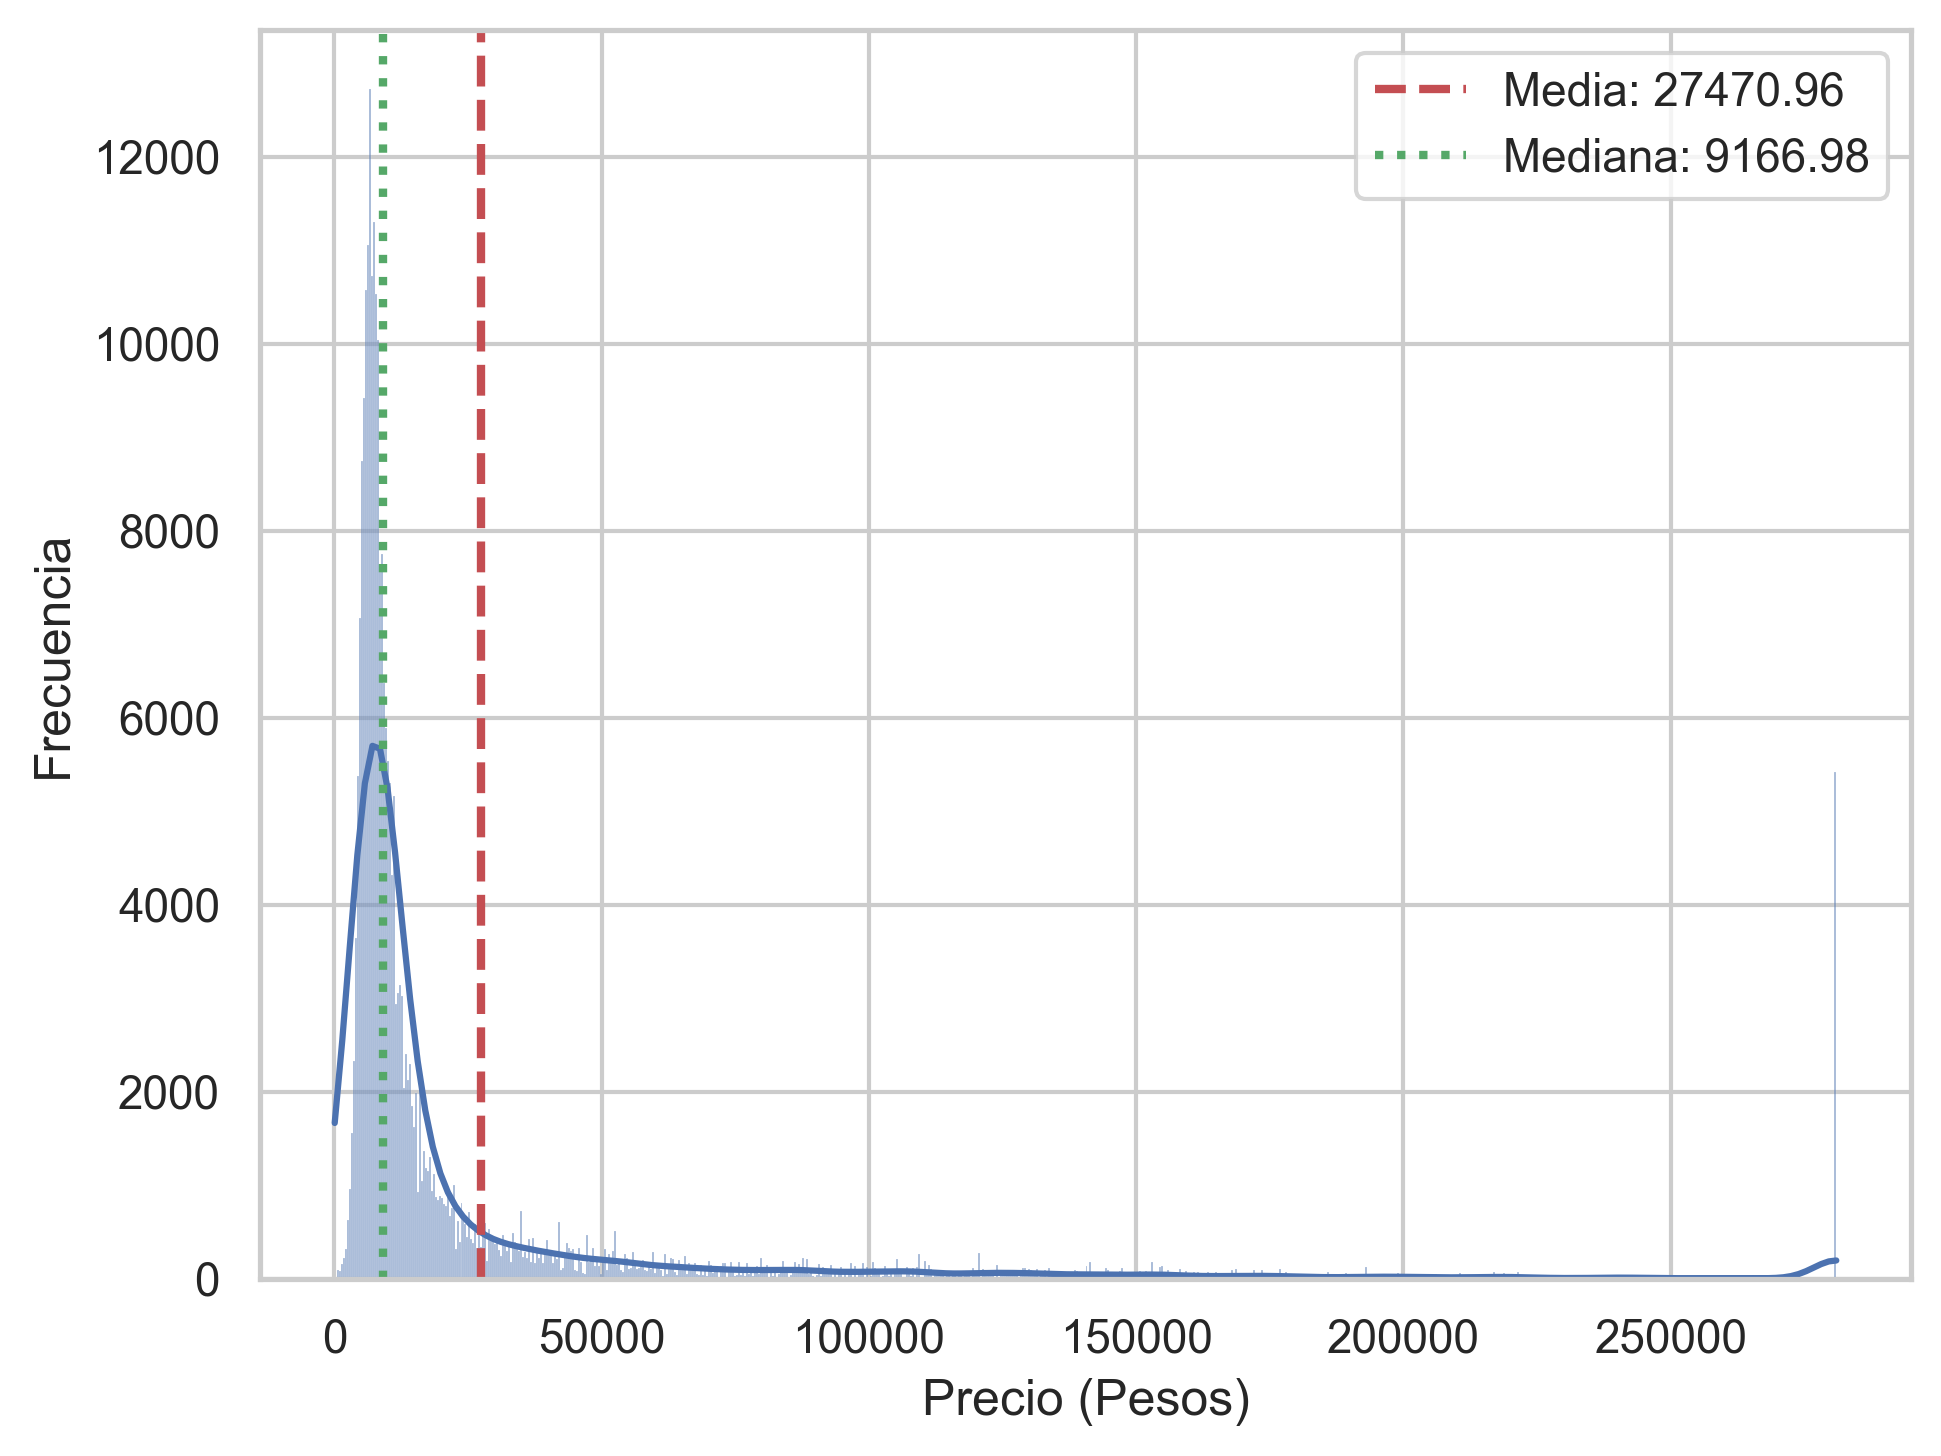
\includegraphics[width=\linewidth]{plots/eda/03-distribucion-precio-clipped.png}
        \caption{Distribución del precio truncada en percentil 98.5. La diferencia media-mediana evidencia asimetría extrema.}
        \label{fig:precio_hist}
    \end{figure}

    \textbf{Correlaciones.} La Figura~\ref{fig:corr} revela correlación entre features de superficie y de habitabilidad (dormitorios, baños, ambientes) con el precio. La antigüedad, en cambio, no correlaciona con el precio. Sorprendentemente, las coordenadas geográficas muestran correlación débil, sugiriendo relaciones altamente no-lineales entre la ubicación y el precio.

    \begin{figure}[H]
        \centering
        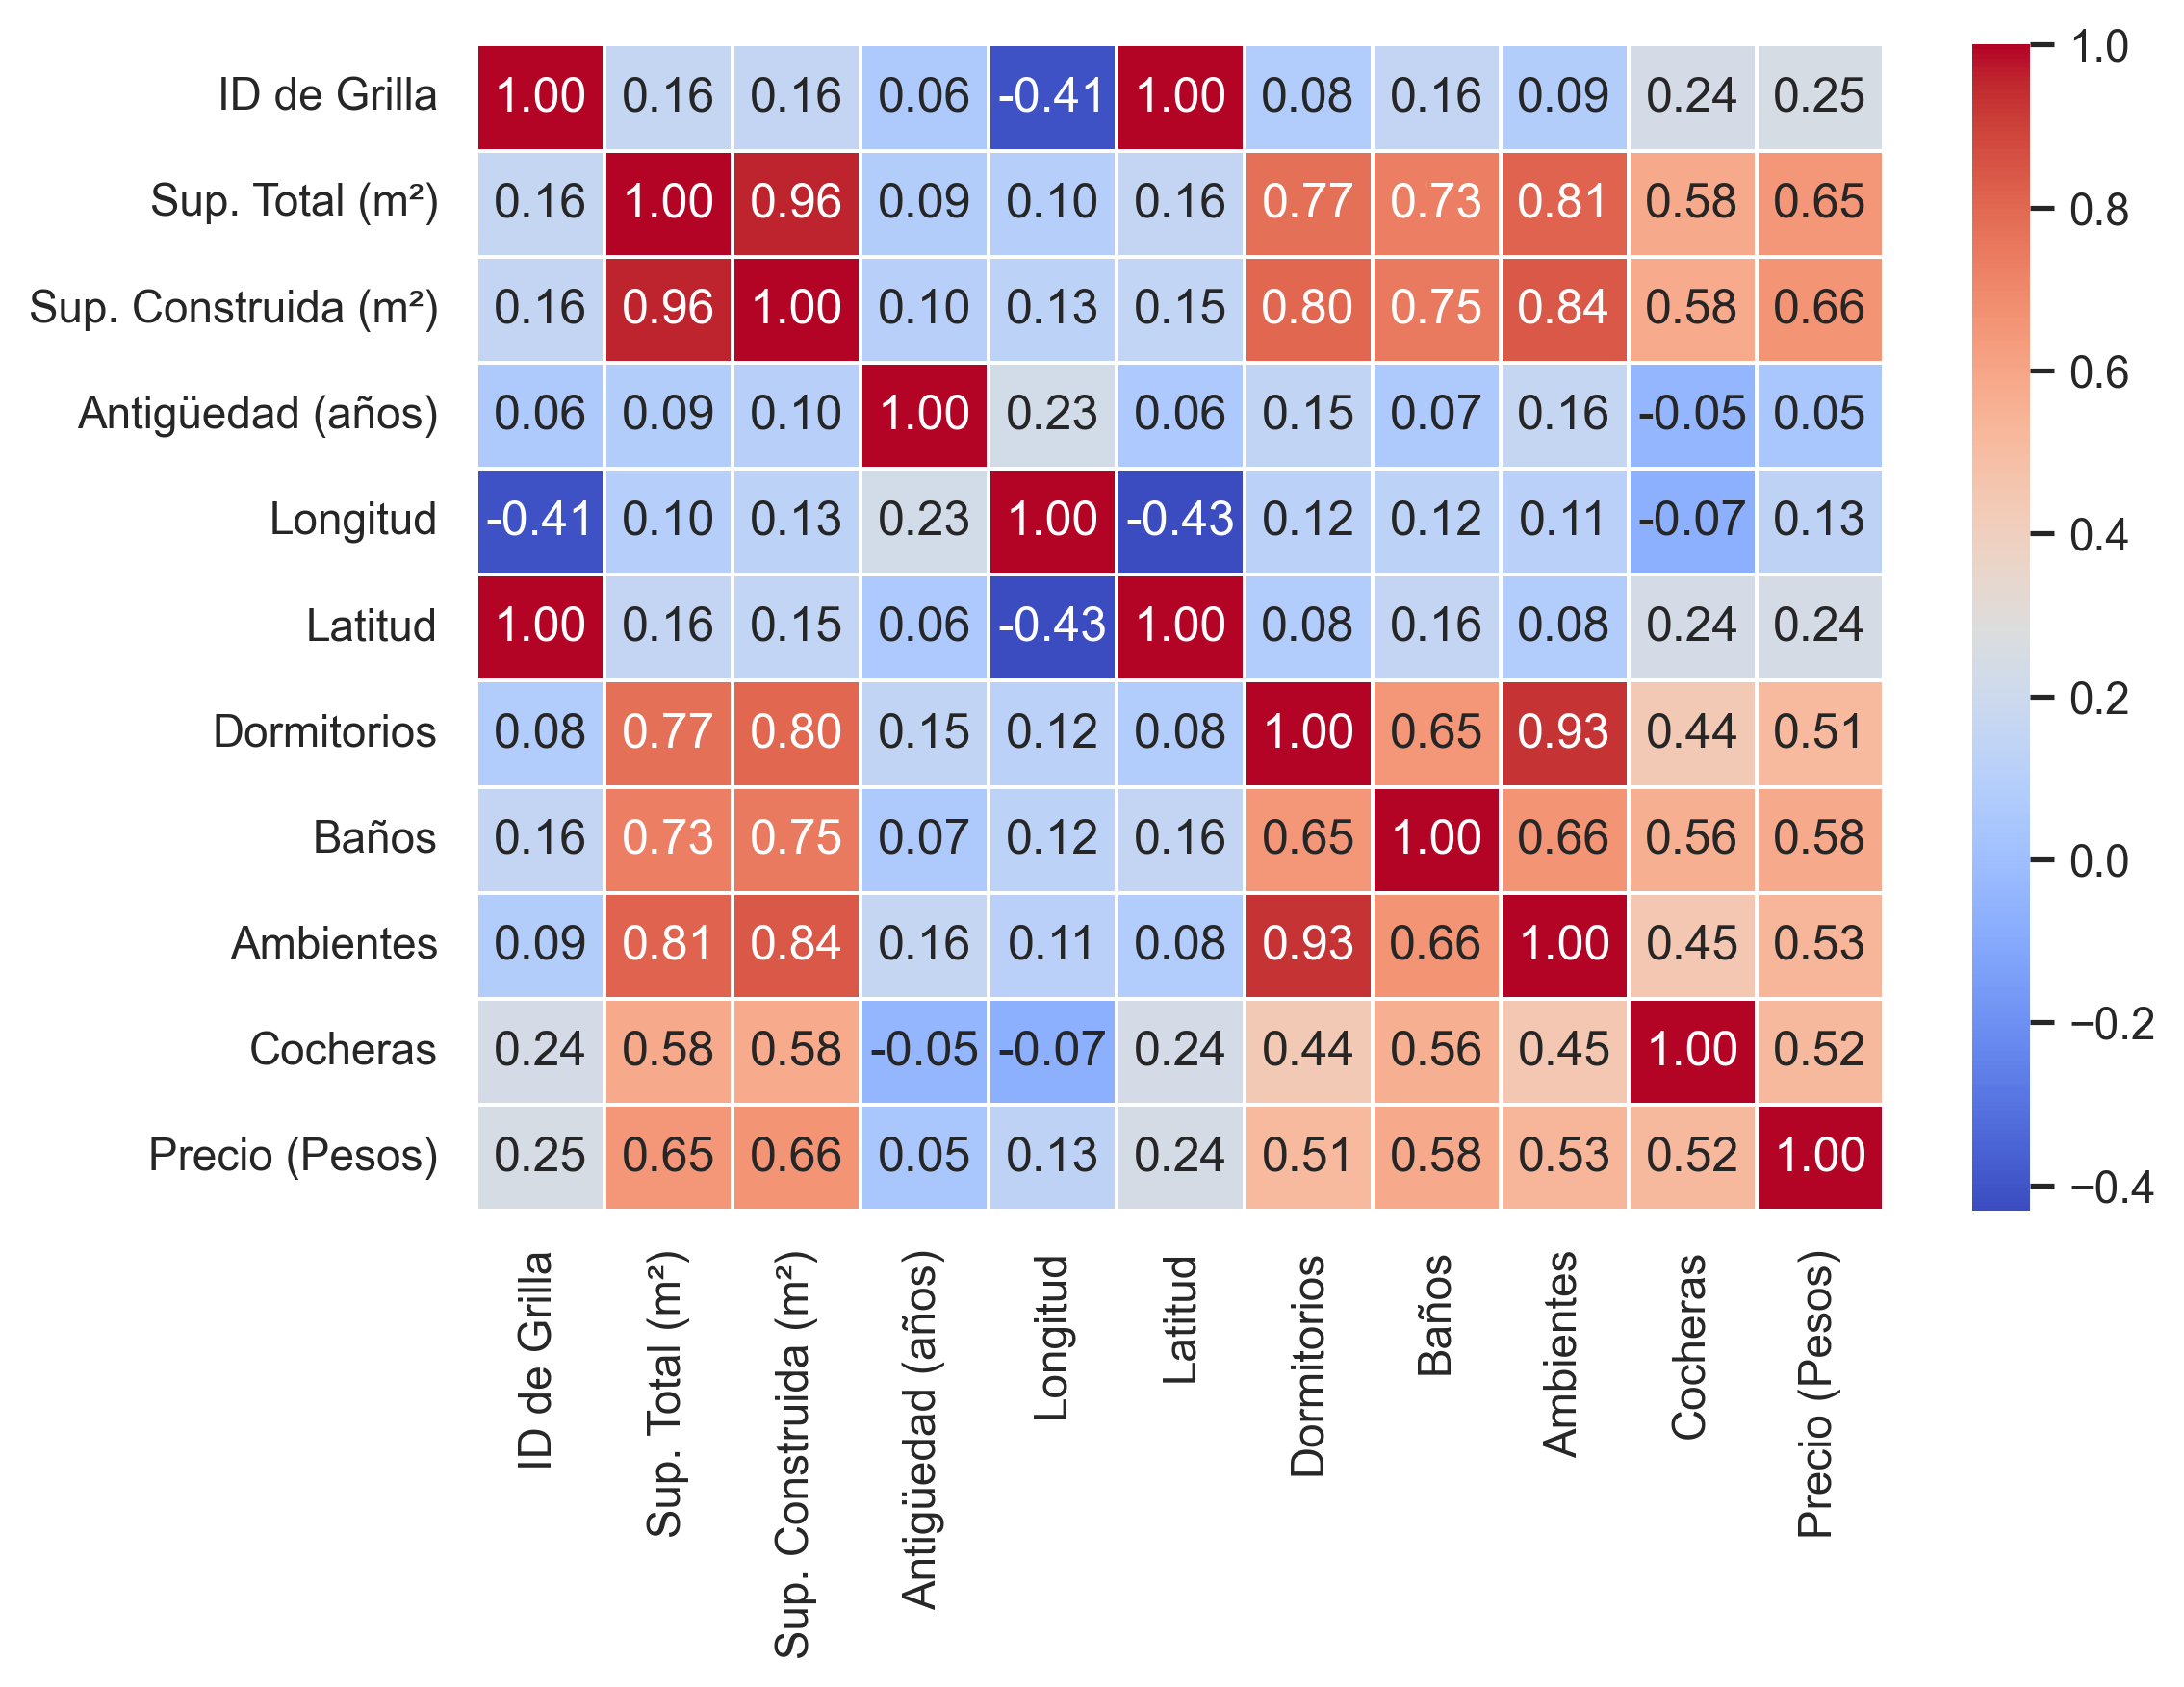
\includegraphics[width=\linewidth]{plots/eda/04-correlation-matrix-std.png}
        \caption{Matriz de correlación de features numéricas. Features de superficie y habilidad muestran alta correlación, mientras que las coordenadas muestran baja correlación lineal.}
        \label{fig:corr}
    \end{figure}

    \textbf{Distribución geográfica.} La Figura~\ref{fig:geoplot} confirma la importancia de la ubicación, a pesar de no tener correlación lineal con el precio: la zona norte y cercana al Río de la Plata concentran los precios altos. Además, hay hexágonos verdosos aislados en el conurbano que probablemente se correspondan con barrios privados y sean difíciles de captar por modelos lineales. Por último, se ven outliers muy amarillos en zonas poder adquisitivo medio que refuerzan la hipótesis de datos erróneos en propiedades con precios extremos.

    \begin{figure}[t]
        \centering
        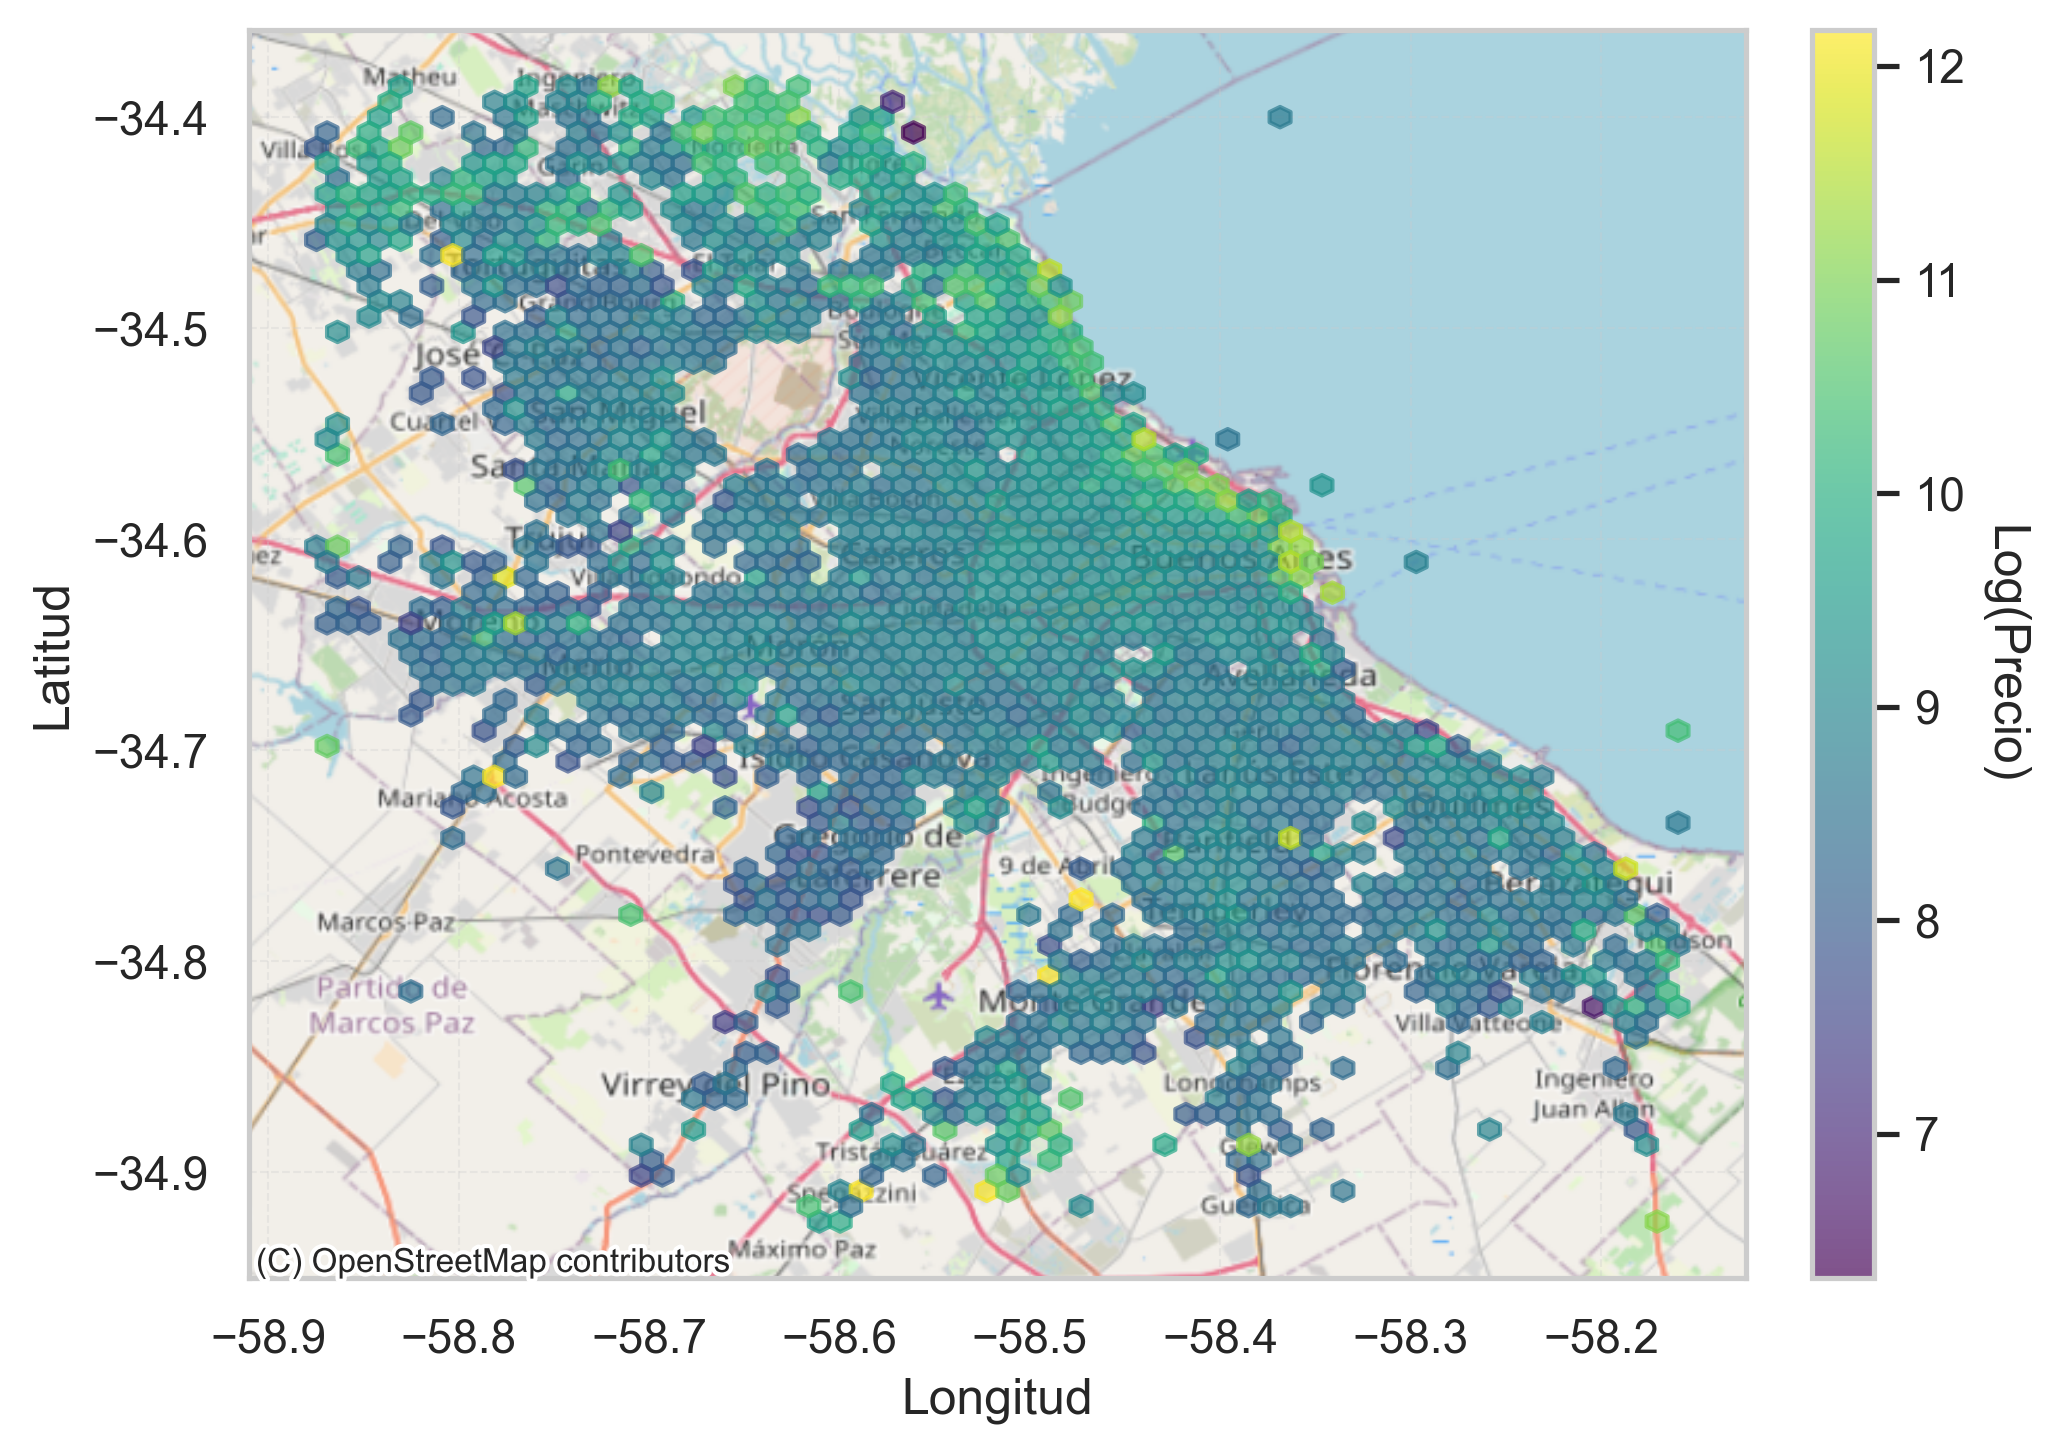
\includegraphics[width=0.9\linewidth]{plots/eda/11-geo-plot.png}
        \caption{Distribución espacial (hexbin, escala log del color). Se observan colores más amarillos hacia el norte y hacia el río.}
        \label{fig:geoplot}
    \end{figure}

    \textbf{PCA.} La Figura~\ref{fig:pca} proyecta propiedades en en las dos primeras componentes principales. Se observa que el precio aumenta notablemente de izquierda a derecha (PC1) y levemente hacia arriba (PC2). Un análisis de contribución de las features a las componentes principales reveló que PC1 está relacionada principalmente con features de superficie y habitabilidad, y PC2 con features de ubicación, lo cual se condice con nuestros análisis hasta el momento.

    \begin{figure}[t]
        \centering
        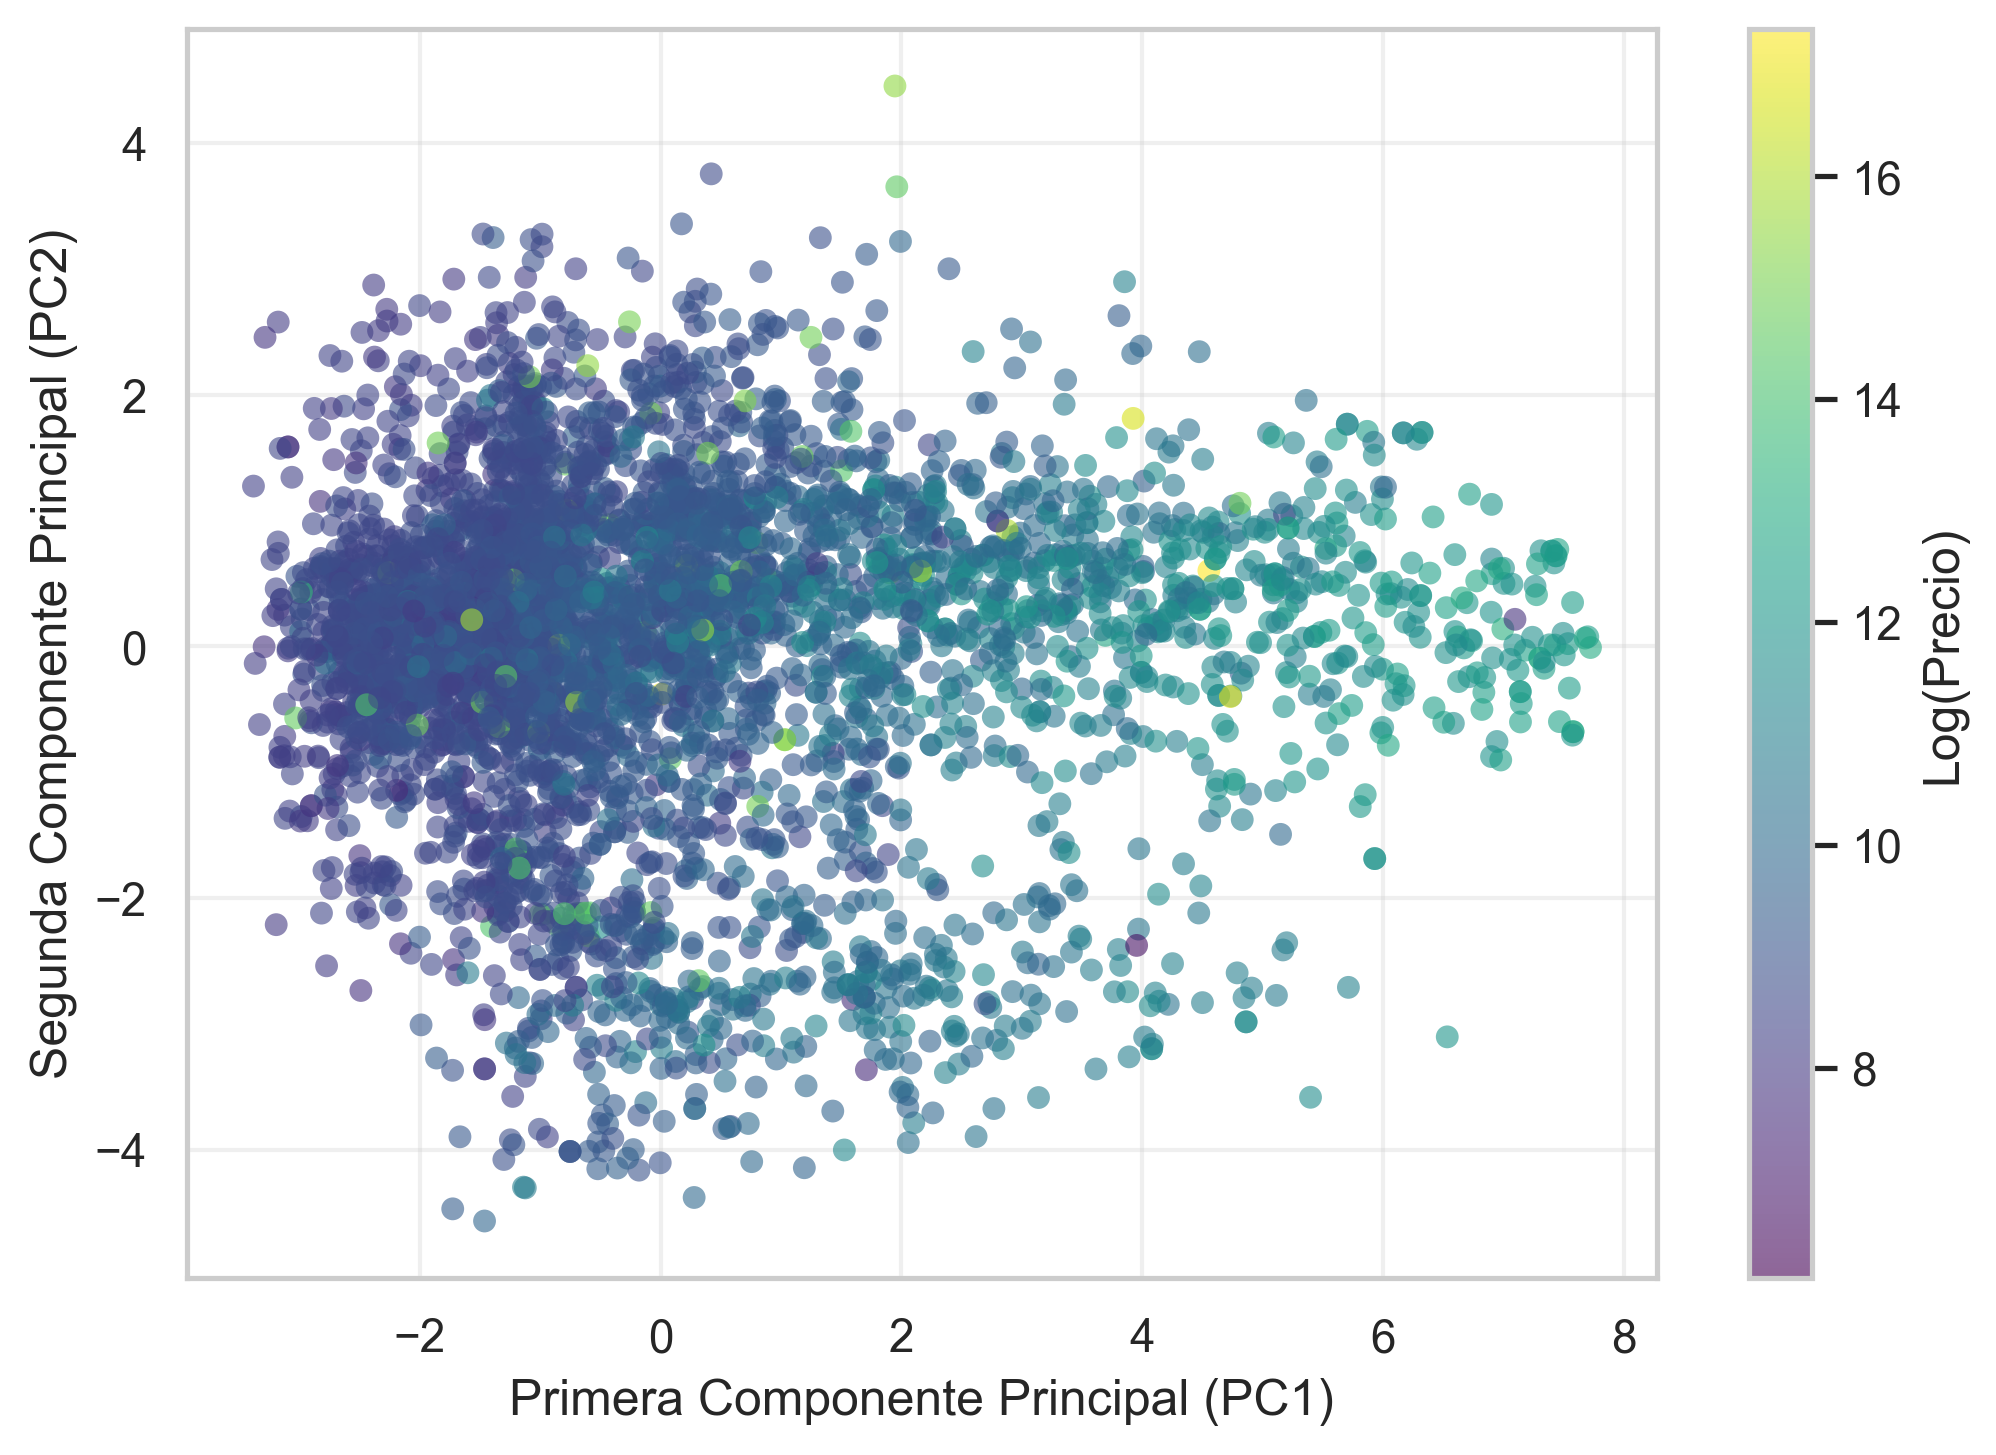
\includegraphics[width=0.9\linewidth]{plots/eda/12-pca-precio.png}
        \caption{Proyección PCA coloreada por log(precio). Se observa un aumento gradual del precio hacia la derecha, sin clusters identificables.}
        \label{fig:pca}
    \end{figure}

    \subsection{Preprocesamiento}

    Se evaluaron tres versiones del dataset: (1) completo, (2) sin el 1.5\% más caro, (3) solo con el 1.5\% más caro. Probando distintas configuraciones sobre los modelos baseline (Dummy, Lasso y XGBoost con configuraciones predeterminadas) se determinaron las configuraciones óptimas:

    \textbf{Árboles:} Imputación por mediana/moda, features creadas (score amenities, densidad habitaciones, ratio baños/dormitorios), ordinal encoding (barrio, ciudad), transformación $\log(\text{precio})$ en el dataset de outliers. Estos modelos requirieron mucho menos preprocesamiento que los lineales.

    \textbf{Lineales/MLP:} Además de imputación y nuevas features, se agregó transformación logarítmica de superficie y antigüedad, estandarización de todas las features numéricas, target encoding (barrio, ciudad), transformación $\log(\text{precio}+1)$ en dataset de outliers.




    \section{Metodología}
    \subsection{Métricas de evaluación}
    Se utilizó el \textbf{Mean Absolute Error (MAE)} como métrica principal:
    \begin{equation}
        \text{MAE} = \frac{1}{n} \sum_{i=1}^{n} |y_i - \hat{y}_i|
    \end{equation}
    Esta elección se tomó por dos razones: (1) interpretabilidad directa como error promedio en pesos, y (2) robustez ante outliers, ya que no eleva el error al cuadrado. Como métrica secundaria se utilizó \textbf{RMSE} ($\sqrt{\frac{1}{n}\sum(y_i - \hat{y}_i)^2}$), que penaliza más fuertemente los errores grandes pero es sensible a los valores extremos identificados en el EDA.
    \subsection{Algoritmos utilizados}
    \subsubsection{Modelos baseline}
    Se evaluaron cuatro modelos base: (1) \textbf{DummyRegressor} (predicción de la mediana), (2) \textbf{Lasso} (regresión lineal con regularización $L_1$), (3) \textbf{Decision Tree}, y (4) \textbf{XGBoost} con parámetros por defecto.
    \subsubsection{Gradient Boosting}
    Se evaluaron dos implementaciones de gradient boosting: \textbf{XGBoost} (\texttt{xgboost}) y \textbf{LightGBM} (\texttt{lightgbm}). Ambos son algoritmos de ensamble que construyen árboles de decisión secuencialmente, donde cada árbol corrige los errores residuales del anterior. En los dos casos se utilizó la función de pérdida predeterminada (MSE).
    \subsubsection{Redes Neuronales}
    Se exploraron redes neuronales feedforward (\texttt{MLPRegressor} de \texttt{sckit-learn}) con múltiples capas ocultas y función de activación \texttt{relu}
    \subsubsection{Modelo híbrido}
    Se desarrolló un \textbf{modelo híbrido} de dos etapas:
    \begin{enumerate}
        \item \textbf{Clasificación}: Un \texttt{XGBClassifier} determina si la propiedad pertenece al segmento de outliers (percentil superior 1,5\%) o al segmento normal.
        \item \textbf{Predicción especializada}: Según la clasificación, se utiliza un \texttt{XGBRegressor} entrenado específicamente en ese segmento.
    \end{enumerate}
    \subsection{Análisis explicativo con SHAP}
    Para interpretar las predicciones del modelo final, se utilizó la librería \textbf{SHAP}. Para cada predicción, SHAP asigna a cada feature $j$ un valor $\phi_j$ que representa su contribución marginal:
    \begin{equation}
        \hat{y}_i = \phi_0 + \sum_{j=1}^{M} \phi_j(x_i)
    \end{equation}
    donde $\phi_0$ es el valor base (predicción promedio del dataset). Se utilizó \texttt{TreeExplainer}, que calcula valores SHAP exactos de forma eficiente aprovechando la estructura de los árboles de decisión.
%----------------------------------------------------------
    \section{Experimentos}
    \subsection{Diseño experimental}
    El dataset provisto está dividido en dos conjuntos independientes: \textbf{dev} y \textbf{test}. Sobre el conjunto dev, todas las comparaciones de modelos se realizaron mediante \textbf{cross-validation} con $k=3$ folds para modelos de árboles y $k=2$ para redes neuronales (debido al mayor costo computacional). El modelo final seleccionado se evaluó sobre el conjunto test.
    \subsection{Estrategia de segmentación del dataset}
    Dada la fuerte asimetría del precio, se entrenaron modelos sobre tres versiones del dataset:
    \begin{itemize}
        \item \textbf{Completo}: todas las observaciones
        \item \textbf{Normal}: excluyendo el 1,5\% más caro (percentil 98,5)
        \item \textbf{Outliers}: solo el 1,5\% más caro
    \end{itemize}
    \subsection{Selección de modelos}
    \subsubsection{Etapa 1: Evaluación de baselines}
    Se evaluaron modelos con parámetros por defecto sobre datos crudos para establecer una línea base.
    \subsubsection{Etapa 2: Evaluación con preprocesamiento}
    Se aplicaron las configuraciones de preprocesamiento óptimas (sección anterior) y se re-evaluaron los modelos, verificando mejoras en MAE.
    \subsubsection{Etapa 3: Búsqueda de hiperparámetros}
    Para XGBoost, LightGBM y MLPRegressor, se realizó \textbf{RandomizedSearchCV} explorando combinaciones de hiperparámetros clave. Los espacios de búsqueda específicos y los hiperparámetros óptimos obtenidos se detallan en el Apéndice (Tablas~\ref{tab:xgb_regressors}-\ref{tab:search_xgb_outliers}). Para el dataset de outliers se utilizó una estrategia de regularización más agresiva (mayor \texttt{min\_child\_weight}, mayor \texttt{reg\_lambda}) dada la menor cantidad de muestras disponibles.
    \subsubsection{Etapa 4: Entrenamiento del clasificador}
    Para el modelo híbrido, se entrenó un XGBClassifier para predecir si una propiedad pertenece al segmento de outliers, optimizando F1-score mediante RandomizedSearchCV. Los hiperparámetros óptimos incluyen \texttt{scale\_pos\_weight}=65.63 para balancear las clases desbalanceadas (Tabla~\ref{tab:xgb_classifier}).
    \subsubsection{Etapa 5: Evaluación final}
    Todos los modelos candidatos (mejor XGBoost, mejor LightGBM, mejor MLP, modelo híbrido) se evaluaron sobre el \textbf{test set} (nunca visto durante entrenamiento ni tuning) para seleccionar el modelo final.
    \subsection{Análisis explicativo}
    Una vez seleccionado el modelo final, se calcularon valores SHAP sobre el test set para:
    \begin{itemize}
        \item Obtener un ranking global de importancia de features
        \item Determinar el impacto de cada amenity sobre el precio
        \item Analizar cómo varía el impacto de cada amenity según la zona geográfica
        \item Graficar el impacto sobre el precio para features continuas y discretas
    \end{itemize}

% ============================================================
% SECCIÓN: RESULTADOS
% ============================================================

    \section{Resultados}

    \subsection{Comparación de modelos}

    Se evaluaron cinco configuraciones de modelos sobre el conjunto de test: (1) \textbf{Baseline}, un XGBoost con parámetros por defecto sin preprocesamiento; (2) \textbf{Baseline + Preprocesamiento}, aplicando el pipeline óptimo; (3) \textbf{XGBoost Optimizado}, con hiperparámetros ajustados mediante RandomizedSearchCV; (4) \textbf{XGBoost Híbrido}, el modelo de dos etapas (clasificador + regresores especializados); y (5) \textbf{Red Neuronal (MLP)}, un MLPRegressor con arquitectura optimizada. Los modelos lineales (Lasso, Ridge) y el DummyRegressor fueron descartados por su rendimiento significativamente inferior.

    La Tabla~\ref{tab:resultados} resume las métricas obtenidas. El modelo híbrido obtiene el mejor MAE (23,314) y MedAE (934), superando ampliamente al resto. Sin embargo, el XGBoost optimizado presenta un RMSE ligeramente menor (294,633 vs 311,949), evidenciando el trade-off entre ambas métricas. Este comportamiento confirma nuestra hipótesis: el modelo híbrido predice con mayor precisión las propiedades del segmento masivo (reflejado en MAE y MedAE), pero comete errores más grandes en outliers extremos, penalizando el RMSE.

    \begin{table}[H]
        \centering
        \begin{tabular}{lccccc}
            \toprule
            \textbf{Métrica} & \textbf{Híbrido} & \textbf{Optimizado} & \textbf{Base+Prep.} & \textbf{Baseline} & \textbf{MLP} \\
            \midrule
            MAE     & \textbf{23,314}  & 45,515    & 86,913   & 89,264   & 120,395 \\
            RMSE    & 311,949          & \textbf{294,633} & 362,433  & 364,441  & 632,914 \\
            R²      & 0.760            & \textbf{0.786}   & 0.676    & 0.672    & 0.011 \\
            MedAE   & \textbf{934}     & 8,360     & 34,746   & 35,022   & 59,782 \\
            \bottomrule
        \end{tabular}
        \caption{Métricas de evaluación en el conjunto de test. En negrita el mejor valor por métrica. El modelo híbrido domina en MAE y MedAE, mientras que XGBoost optimizado obtiene mejor RMSE y R².}
        \label{tab:resultados}
    \end{table}

    La Figura~\ref{fig:comparacion} visualiza esta comparación. Es notable la excepcional performance del modelo híbrido en MedAE (mediana del error absoluto), siendo casi 9 veces menor que el XGBoost optimizado. Esto demuestra que el 50\% de las predicciones del modelo híbrido tienen un error menor a \$934, ilustrando el fuerte impacto de los outliers sobre las métricas basadas en la media.

    \begin{figure}[t]
        \centering
        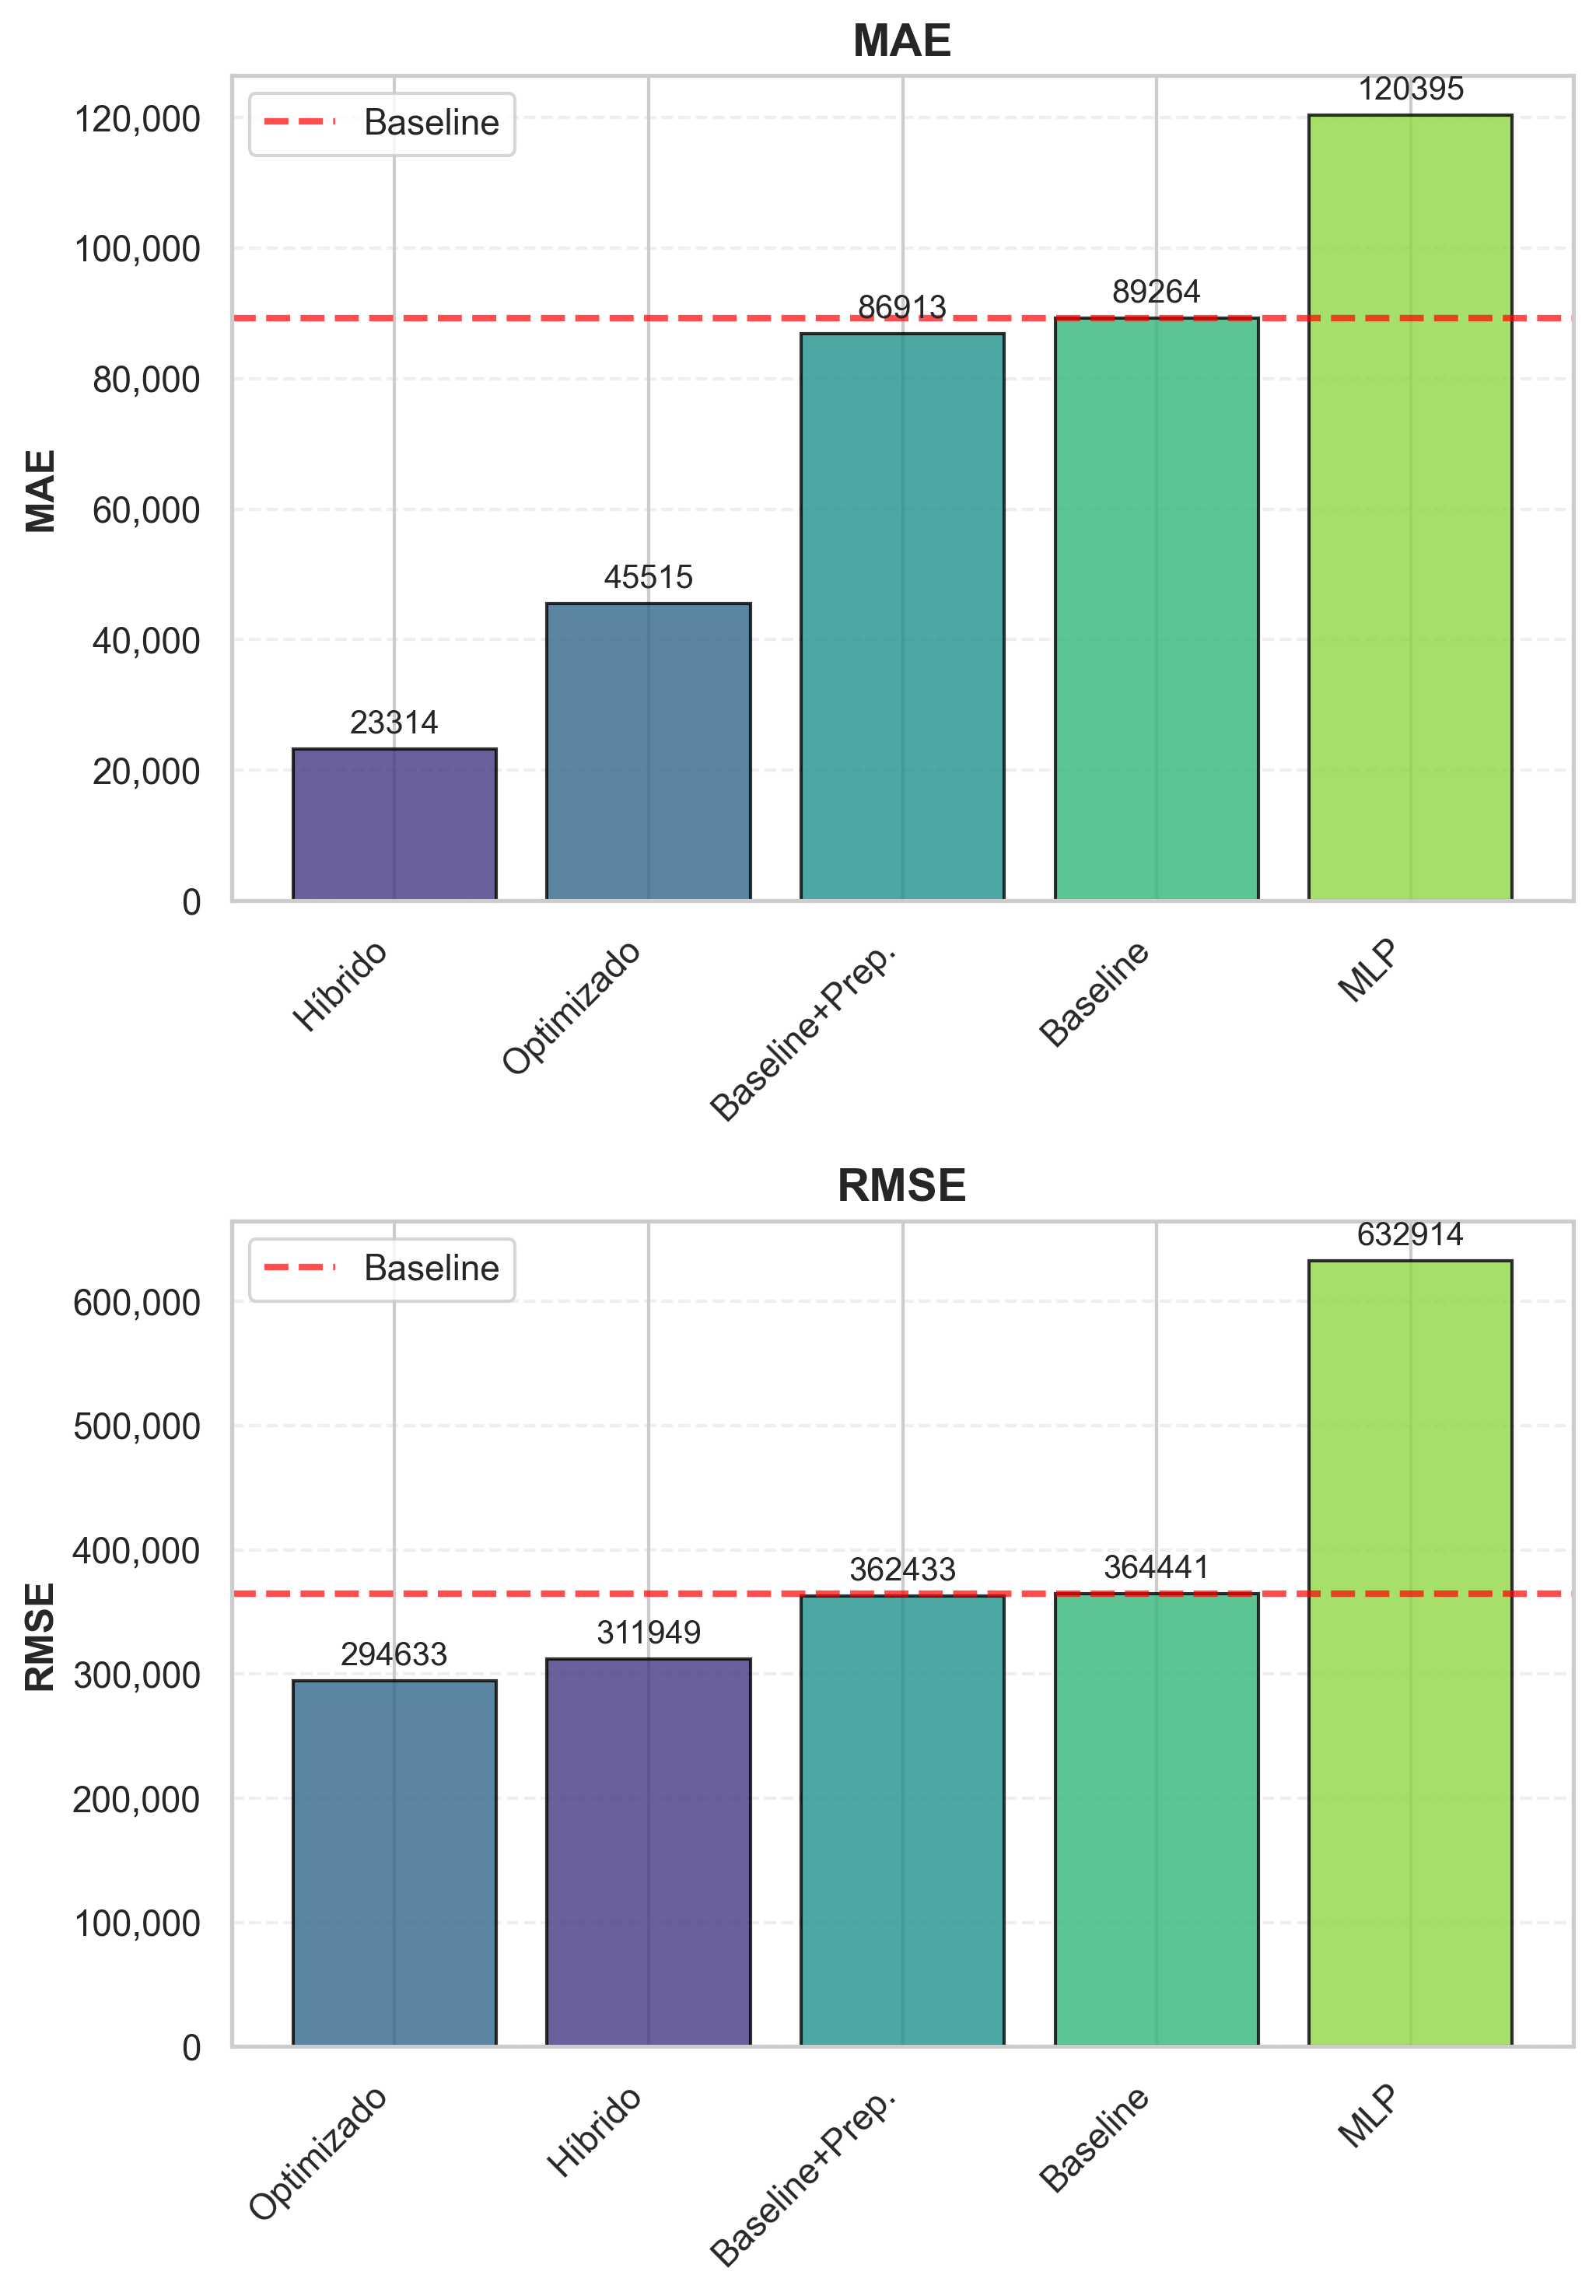
\includegraphics[width=\linewidth]{plots/01-comparacion-final.png}
        \caption{Comparación de MAE y RMSE entre modelos. El modelo híbrido obtiene el menor MAE, mientras que XGBoost optimizado logra el menor RMSE.}
        \label{fig:comparacion}
    \end{figure}

    Un resultado inesperado es el pobre desempeño del MLP, incluso inferior al baseline sin preprocesamiento. Esto refleja la conocida superioridad de los modelos de gradient boosting en datos tabulares estructurados: XGBoost maneja naturalmente features heterogéneas (numéricas, categóricas, booleanas), captura interacciones complejas sin requerir feature engineering manual, y es robusto a diferentes escalas. Las redes neuronales, en cambio, requieren mayor volumen de datos, arquitecturas cuidadosamente diseñadas y son más sensibles a la distribución de las features para alcanzar rendimiento competitivo en este tipo de problemas.

    \subsection{Análisis de predicciones}

    La Figura~\ref{fig:scatter} muestra el scatter plot de predicciones vs valores reales del modelo híbrido en escala logarítmica. La mayoría de los puntos se alinean a lo largo de la diagonal, indicando buena capacidad predictiva general. Sin embargo, se identifican dos nubes anómalas alejadas de la diagonal:

    \begin{itemize}
        \item \textbf{Subestimación extrema} (abajo-derecha): Propiedades con precios reales entre \$1,000,000 y \$20,000,000 que fueron predichas entre \$10,000 y \$100,000. Corresponden a propiedades de ultra-lujo que el modelo no logra capturar.
        \item \textbf{Sobreestimación extrema} (arriba-izquierda): Propiedades con precios reales entre \$5,000 y \$10,000 predichas entre \$1,000,000 y \$10,000,000. Posiblemente son propiedades con características atípicas (amenities de lujo en zonas económicas) o errores en los datos originales.
    \end{itemize}

    Este patrón confirma nuestra hipótesis central: el modelo predice con alta precisión la gran mayoría de las propiedades (segmento masivo), pero falla sistemáticamente en casos extremos que distorsionan el RMSE.

    \begin{figure}[H]
        \centering
        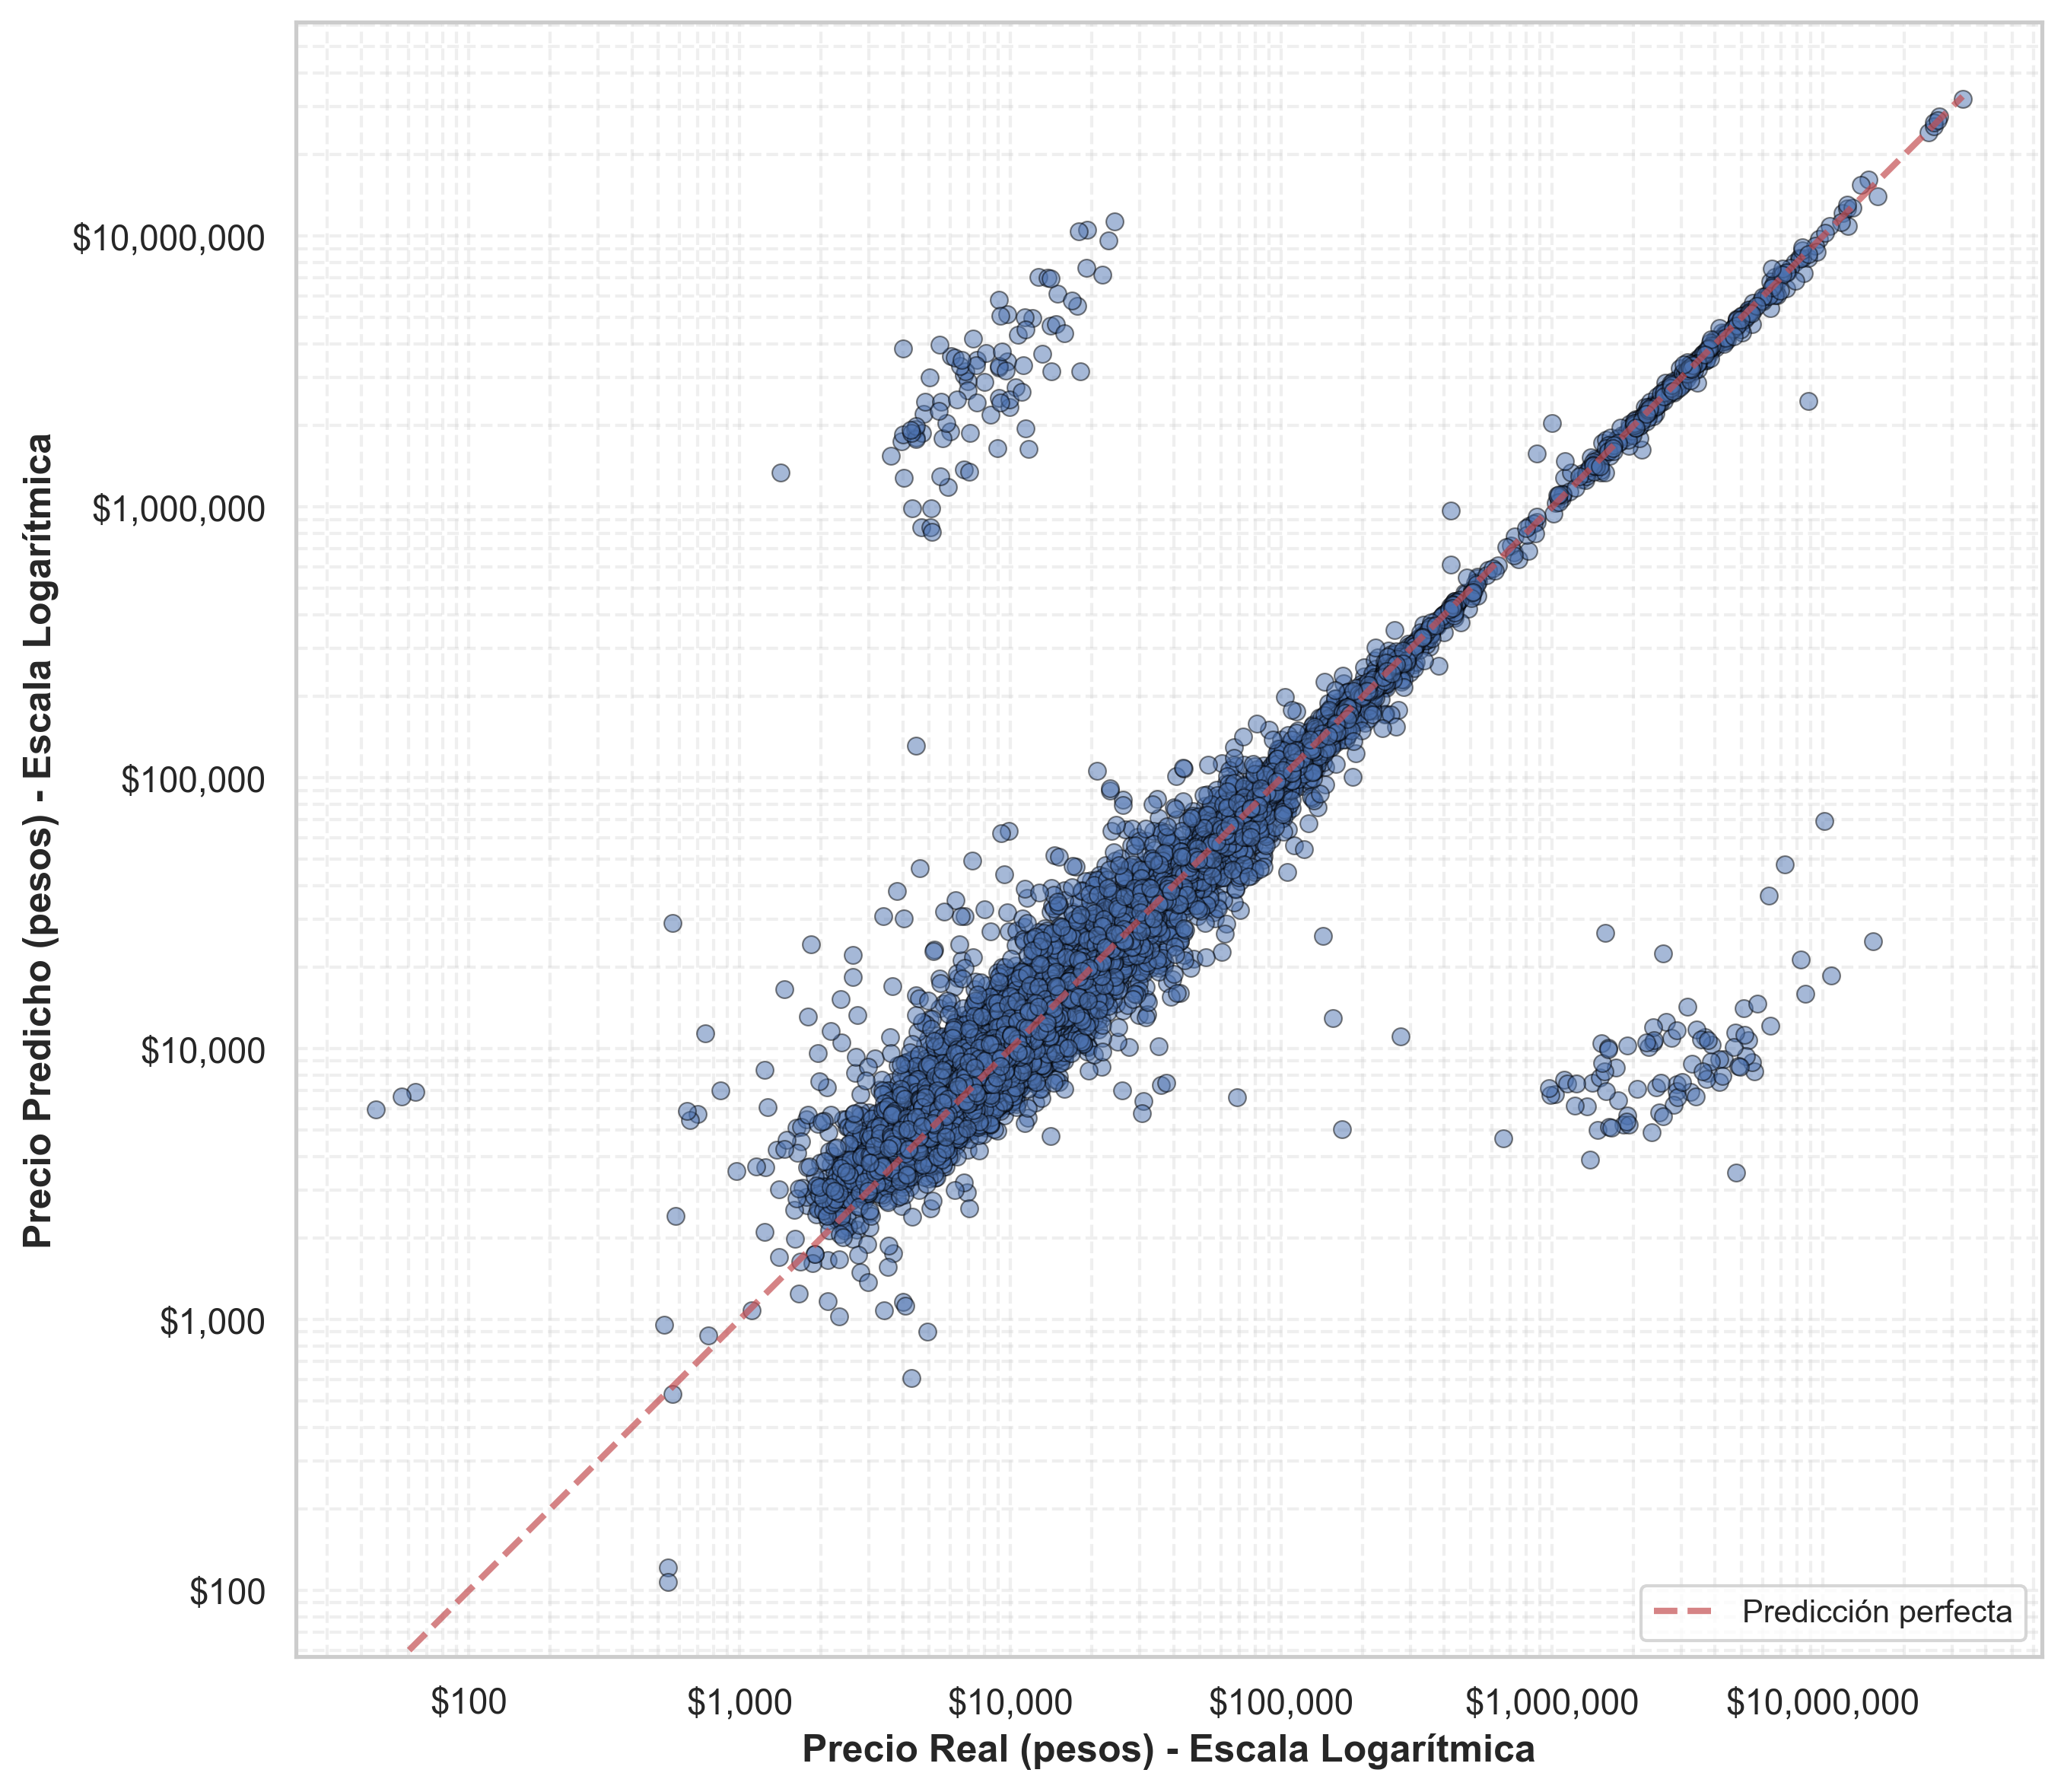
\includegraphics[width=0.85\linewidth]{plots/02-predictions-scatter.png}
        \caption{Predicciones vs valores reales (escala logarítmica). La diagonal indica predicción perfecta. Las nubes alejadas corresponden a outliers sub/sobreestimados.}
        \label{fig:scatter}
    \end{figure}

    \subsection{Análisis de overfitting}

    Los modelos de XGBoost presentan una brecha notable entre las métricas de entrenamiento y test, lo cual podría sugerir sobreajuste. Sin embargo, el análisis de las curvas de aprendizaje revela un comportamiento saludable: si bien la pérdida en train continúa decreciendo, la pérdida en validación decrece asintóticamente sin aumentar. Esto indica que, aunque el modelo se ajusta progresivamente mejor a los datos de entrenamiento, esto no degrada su capacidad de generalización. La regularización implícita de XGBoost (max\_depth, min\_child\_weight, subsampling) mitiga efectivamente el overfitting.

% ============================================================
% SECCIÓN: ANÁLISIS EXPLICATIVO
% ============================================================

    \section{Análisis Explicativo}

    Para interpretar las predicciones del modelo final, se calcularon valores SHAP sobre el conjunto de test, permitiendo cuantificar la contribución de cada feature a cada predicción individual.

    \subsection{Importancia global de features}

    La Figura~\ref{fig:importance} muestra el ranking de importancia SHAP. La \textbf{superficie construida} domina claramente, seguida por baños, gimnasio, longitud, ID de grilla y cocheras. Este resultado valida los hallazgos del EDA: el tamaño de la propiedad (superficie), la ubicación geográfica (longitud, ID grilla) y las características de habitabilidad (baños, ambientes) son los principales drivers del precio. Las amenities, con excepción de gimnasio y pileta, tienen un rol secundario en la formación de precios.

    \begin{figure}[H]
        \centering
        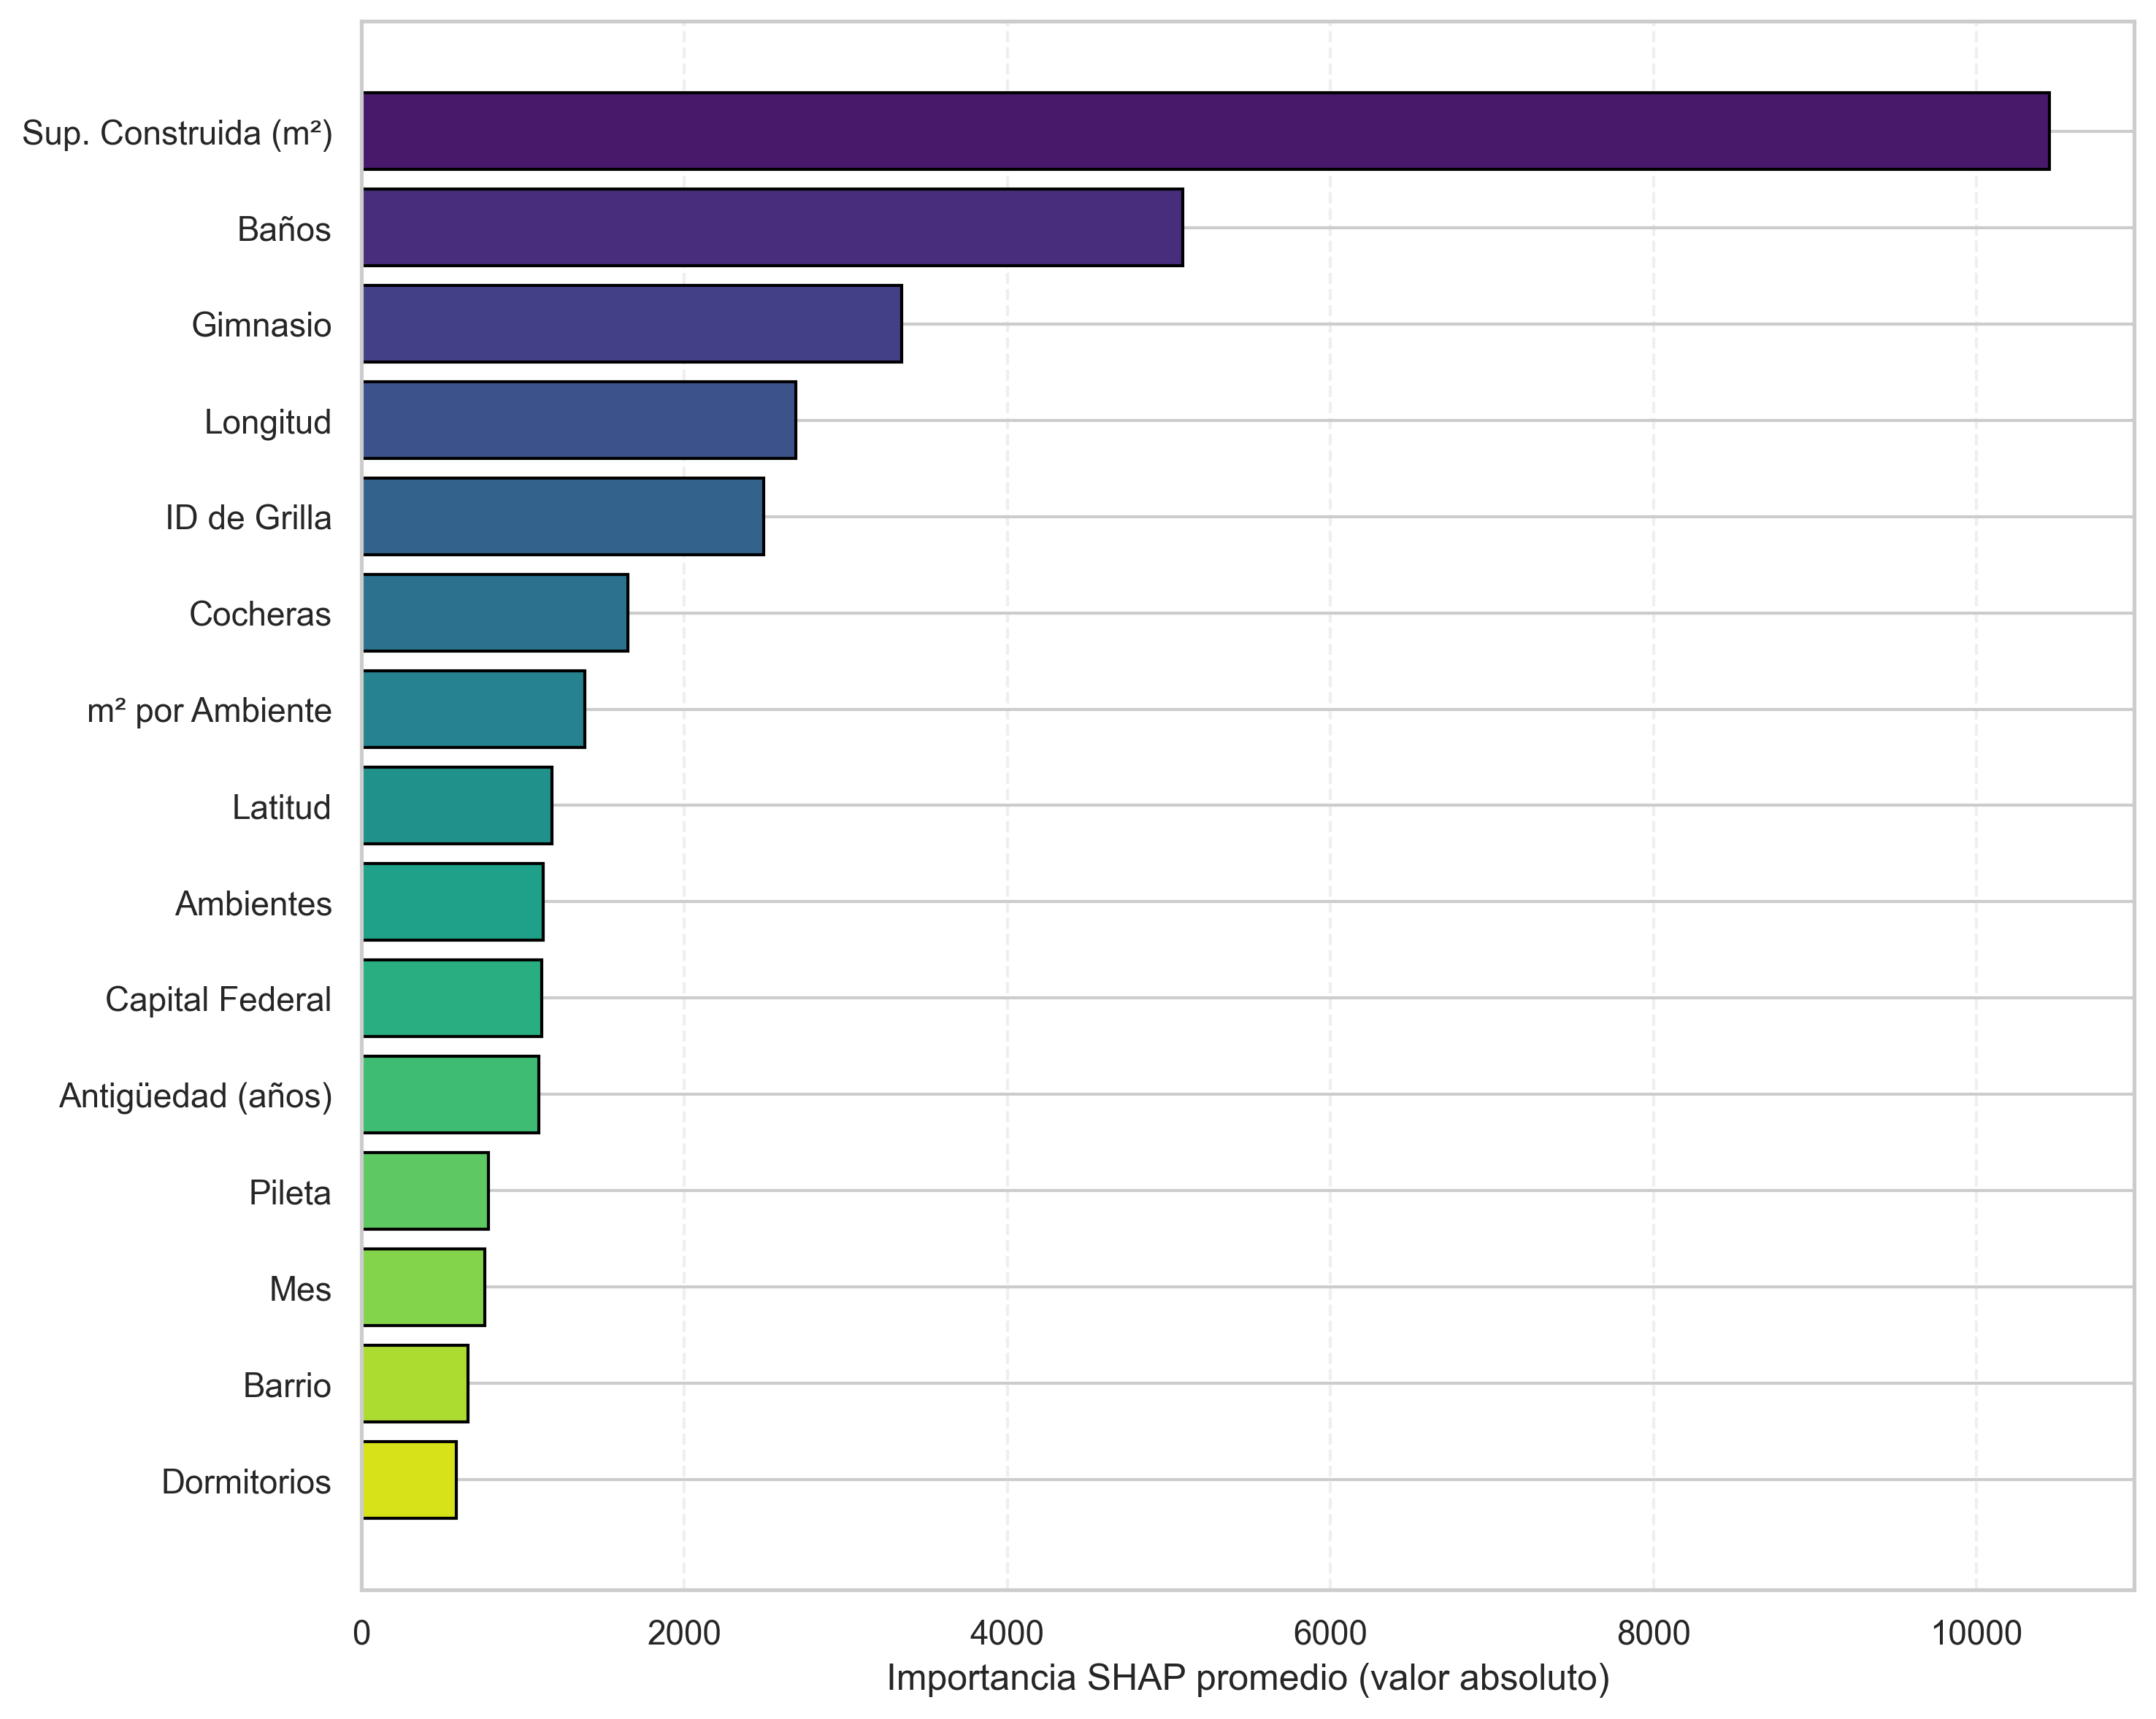
\includegraphics[width=0.9\linewidth]{plots/analisis-explicativo/01-feature-importance.png}
        \caption{Importancia SHAP de features. La superficie construida es el predictor dominante, seguida por características de habitabilidad y ubicación.}
        \label{fig:importance}
    \end{figure}

    \subsection{Impacto de amenities}

    La Figura~\ref{fig:amenities} cuantifica el impacto promedio de cada amenity sobre el precio. El \textbf{gimnasio} presenta el mayor impacto positivo, seguido de amoblado y pileta. Este orden refleja tanto la escasez relativa de estas amenities como su valoración por el mercado.

    \begin{figure}[H]
        \centering
        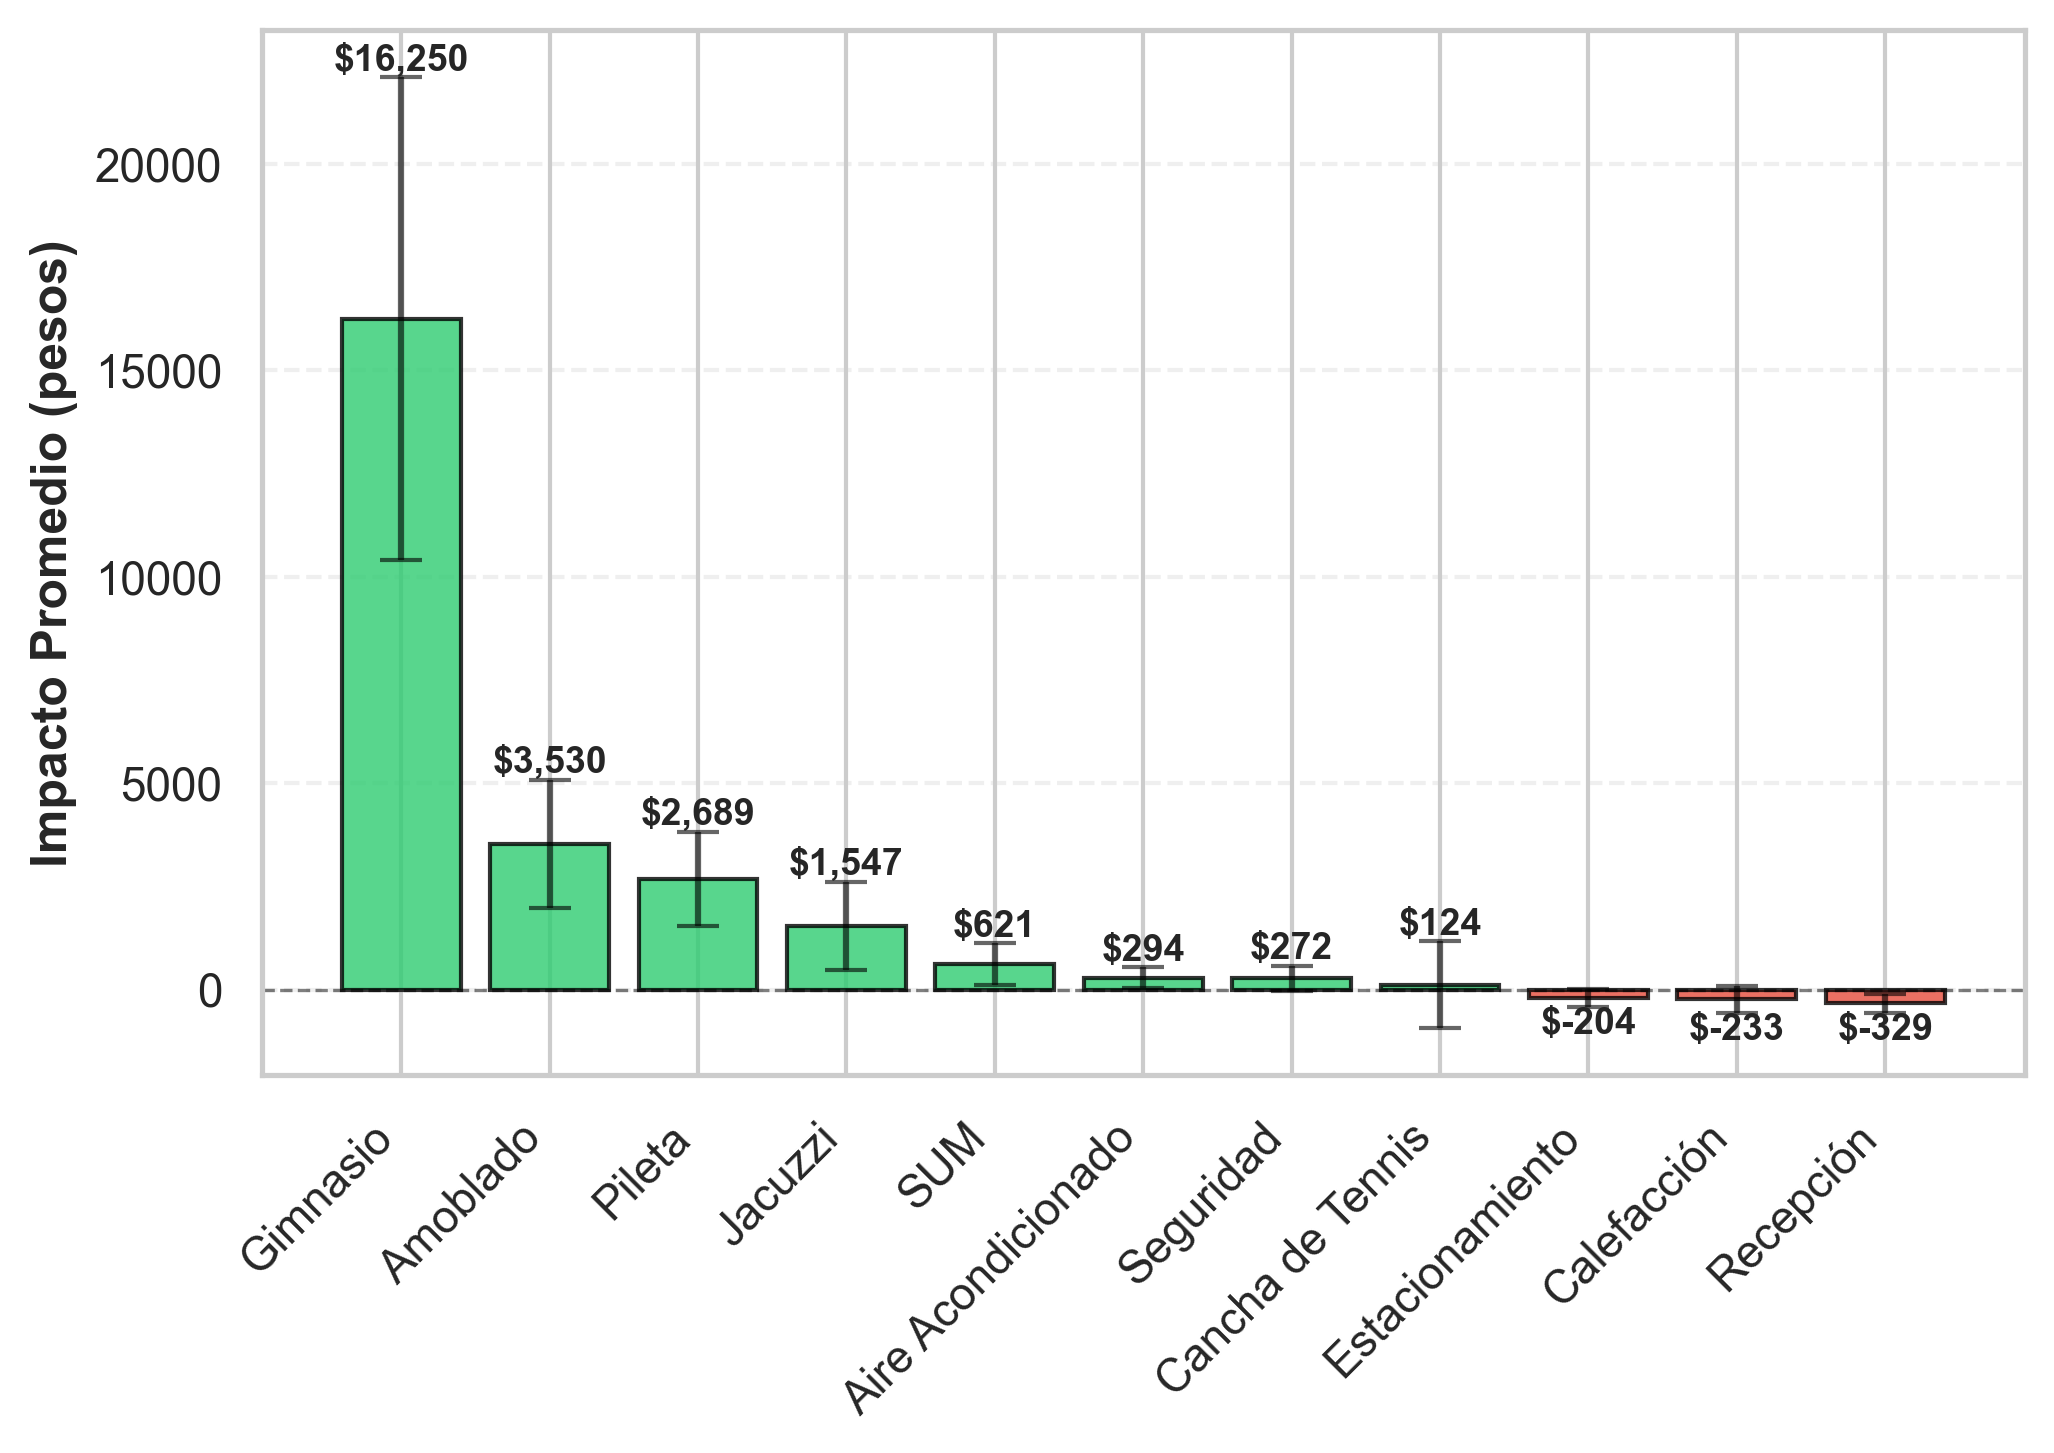
\includegraphics[width=0.9\linewidth]{plots/analisis-explicativo/02-amenities-impact.png}
        \caption{Impacto SHAP promedio de cada amenity sobre el precio de alquiler.}
        \label{fig:amenities}
    \end{figure}

    El análisis por zona geográfica (Figura~\ref{fig:amenities_zona}) revela heterogeneidad en la valoración de amenities. Capital Federal y Zona Norte muestran impactos significativamente mayores que otras localidades, especialmente para gimnasio, pileta y jacuzzi. Esto sugiere que las amenities son un diferenciador de precio principalmente en mercados de alto poder adquisitivo, mientras que en zonas más económicas su influencia es marginal.

    \begin{figure}[H]
        \centering
        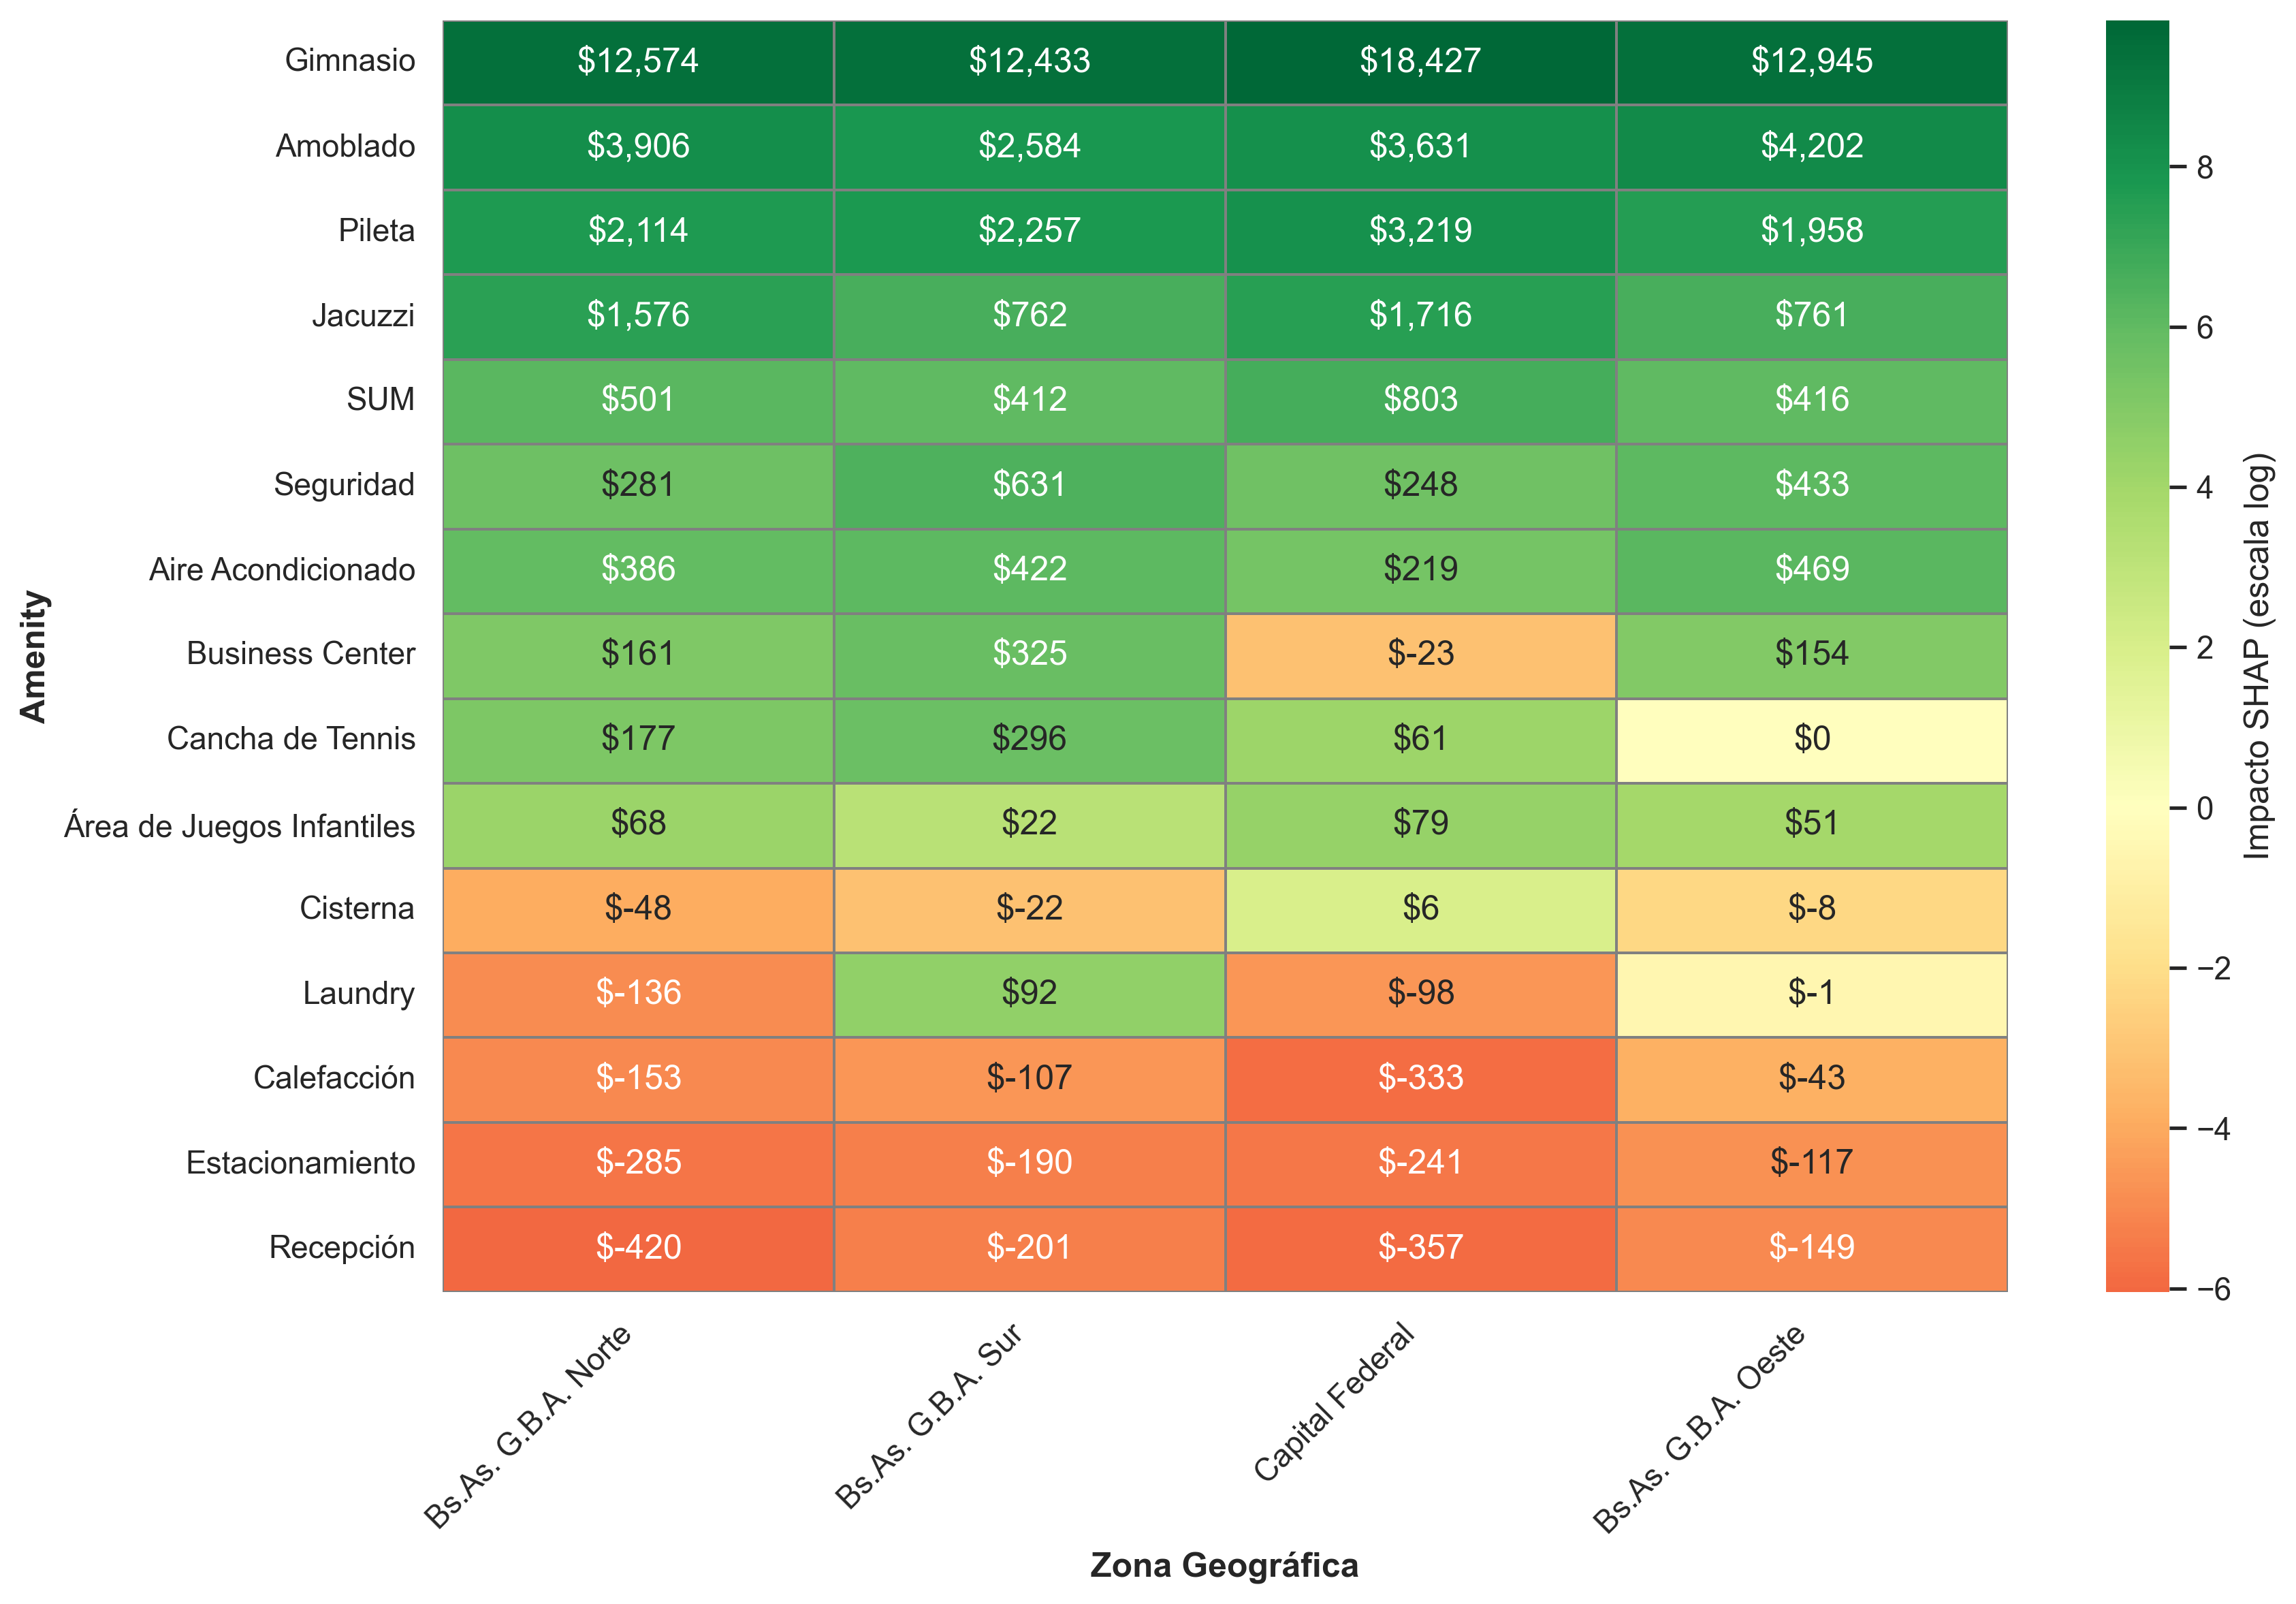
\includegraphics[width=\linewidth]{plots/analisis-explicativo/03-amenities-impact-per-state.png}
        \caption{Impacto de amenities por zona geográfica. Capital Federal y Zona Norte muestran mayor sensibilidad a las amenities.}
        \label{fig:amenities_zona}
    \end{figure}

    \subsection{Efectos de features continuas}

    La Figura~\ref{fig:continuas} muestra los gráficos de dependencia SHAP para las features continuas más relevantes. La \textbf{superficie construida} exhibe una relación monotónica positiva clara: a mayor superficie, mayor precio. La \textbf{longitud} presenta un comportamiento particular: relativamente estable entre -58.9 y -58.5, con un pico pronunciado alrededor de -58.35, que probablemente corresponde a desarrollos inmobiliarios premium como Nordelta u otras zonas de countries.

    \begin{figure}[H]
        \centering
        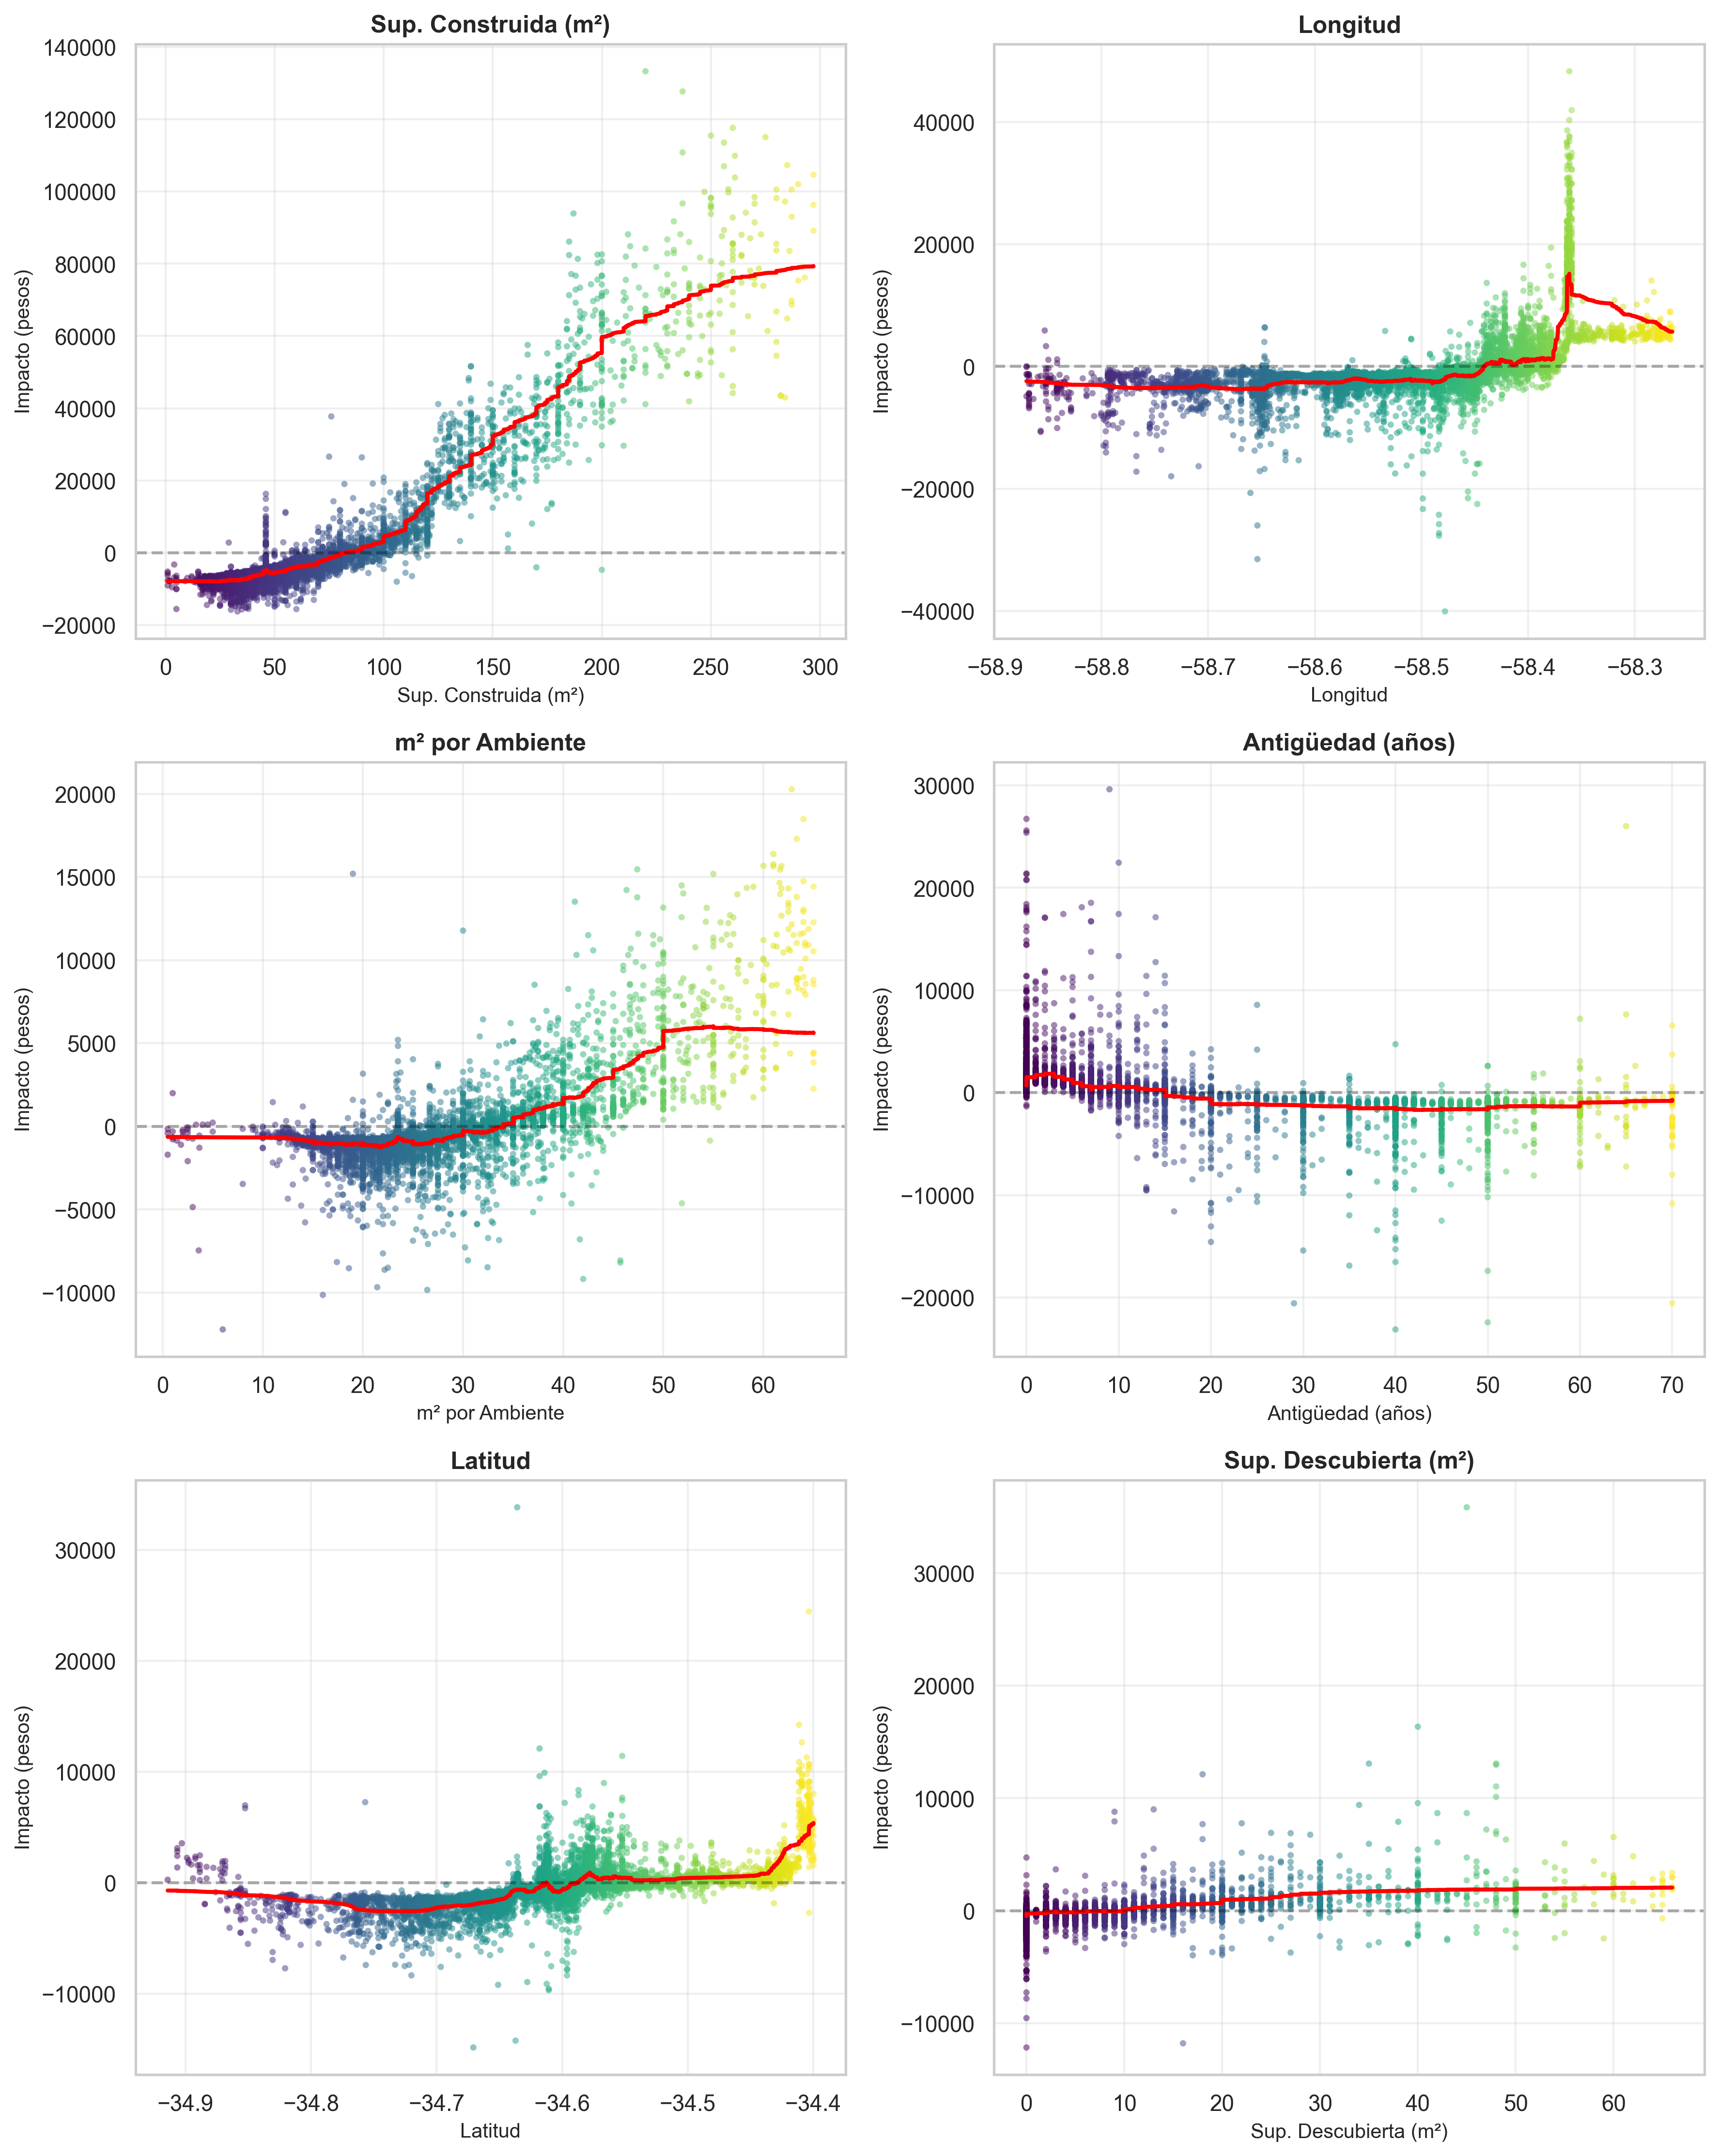
\includegraphics[width=\linewidth]{plots/analisis-explicativo/06-continuous-feats-impact.png}
        \caption{Gráficos de dependencia SHAP para features continuas. Superficie muestra relación monotónica positiva; longitud presenta un pico en zonas premium.}
        \label{fig:continuas}
    \end{figure}

    \subsection{Efectos de features discretas}

    La Figura~\ref{fig:discretas} analiza el impacto de variables discretas. La \textbf{cantidad de baños} tiene un efecto fuertemente positivo, especialmente al pasar de 3 a 4+ baños, donde el incremento en precio es sustancial. Los \textbf{ambientes} muestran un patrón similar: el salto de 4 a 5+ ambientes genera un aumento marcado en el precio predicho. Estos umbrales probablemente marcan la transición hacia propiedades de categoría premium.

    \begin{figure}[H]
        \centering
        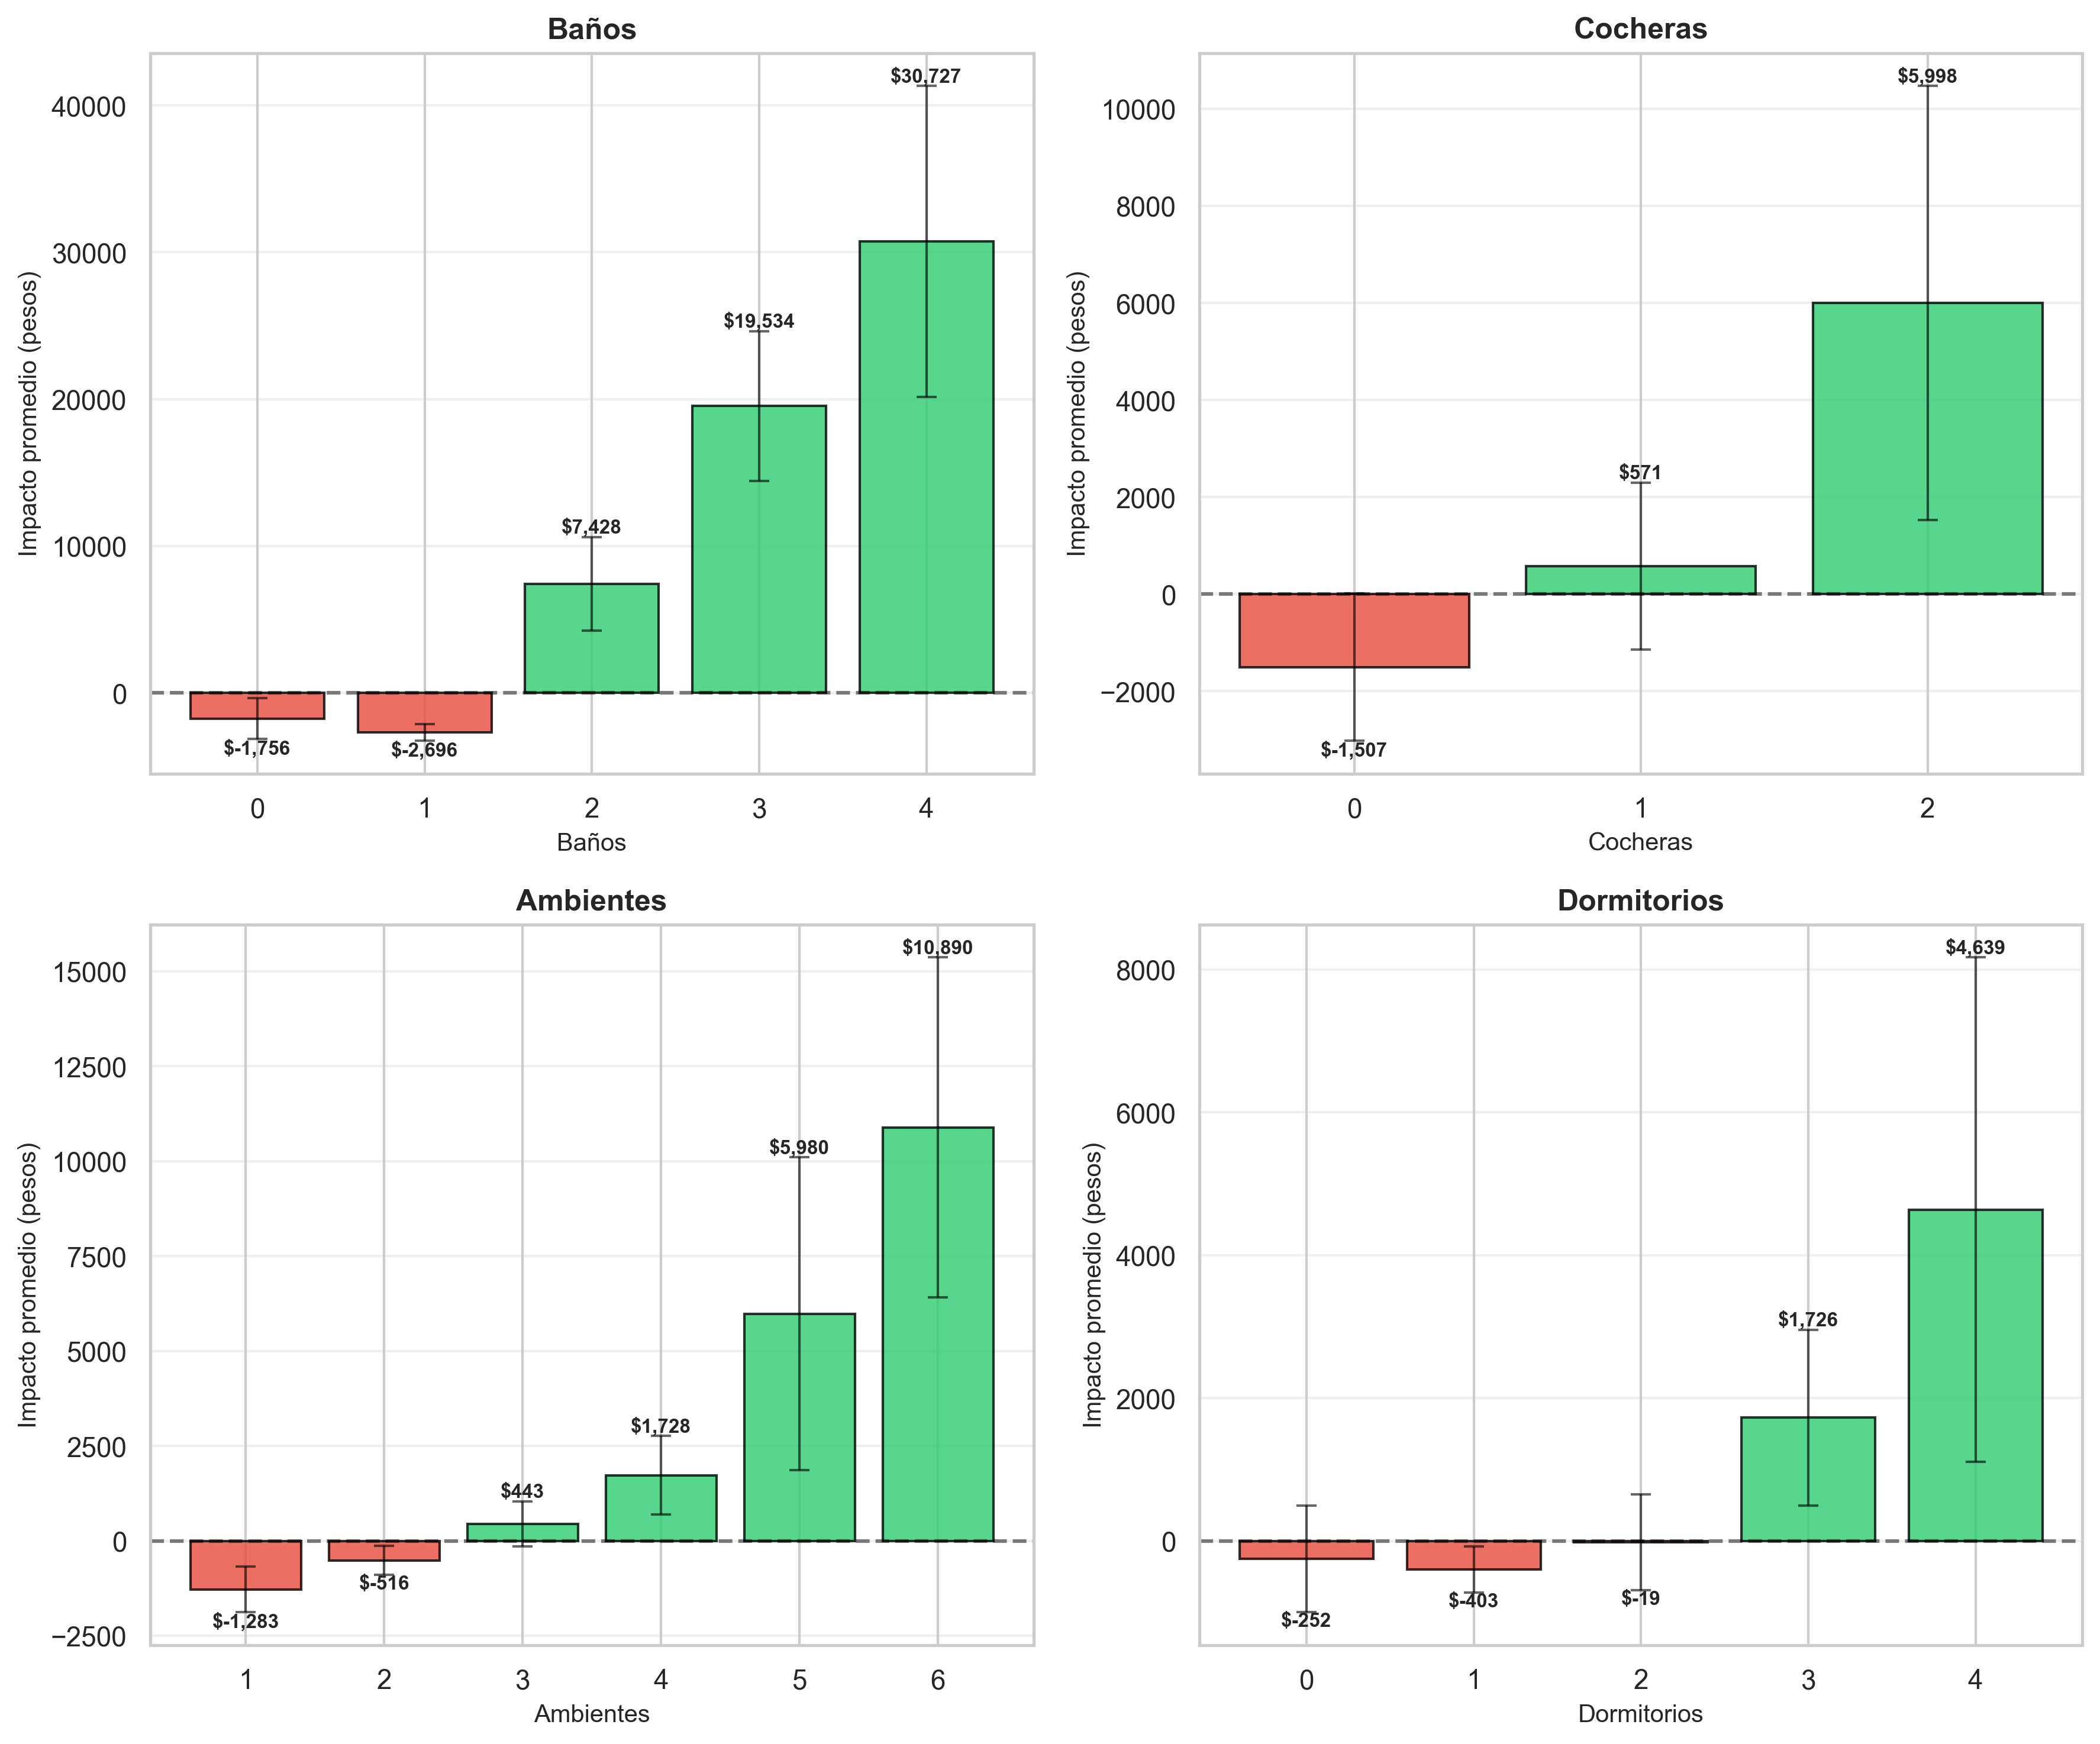
\includegraphics[width=\linewidth]{plots/analisis-explicativo/07-discrete-feats-impact.png}
        \caption{Impacto SHAP de features discretas. Baños y ambientes muestran efectos no lineales con saltos significativos en categorías altas.}
        \label{fig:discretas}
    \end{figure}


% ============================================================
% SECCIÓN: CONCLUSIÓN Y TRABAJO FUTURO
% ============================================================
    \section{Conclusiones}
    Este trabajo abordó la predicción de precios de alquiler en el AMBA utilizando un dataset de 50,000 publicaciones de Mercado Libre. El análisis exploratorio reveló dos desafíos fundamentales: (1) una distribución de precios extremadamente asimétrica con outliers que distorsionan las métricas, y (2) efectos espaciales no lineales donde la ubicación impacta el precio de forma contextual, no simplemente por coordenadas. Estas observaciones guiaron el diseño de un modelo híbrido que segmenta el mercado en propiedades ``normales'' y ``outliers'', aplicando regresores especializados para cada segmento.

    Los resultados demuestran la superioridad de XGBoost sobre modelos lineales y redes neuronales en datos tabulares estructurados, confirmando hallazgos de la literatura reciente. El modelo híbrido logró el mejor MAE (23,314) y MedAE (934), mientras que el XGBoost optimizado obtuvo mejor RMSE (294,633). Este trade-off refleja una tensión inherente al problema: optimizar para el error promedio (MAE) beneficia al segmento masivo del mercado, mientras que minimizar errores cuadráticos (RMSE) prioriza reducir errores extremos en propiedades de lujo. Consideramos que el modelo híbrido es la mejor elección para aplicaciones prácticas, dado que la mayoría de las consultas corresponderían a propiedades del segmento masivo. El análisis SHAP confirmó que superficie, ubicación y características de habitabilidad son los principales drivers del precio, mientras que las amenities tienen mayor impacto en zonas de alto poder adquisitivo.

    \textbf{Trabajo futuro.} Identificamos tres direcciones prometedoras: (1) \textit{Modelado basado en PCA}: utilizar las componentes principales como features podría capturar estructura latente del mercado y reducir dimensionalidad sin perder información predictiva. (2) \textit{Mejora en predicción de outliers}: las ``nubes'' del scatter plot (propiedades extremadamente sub/sobreestimadas) merecen análisis específico; identificar sus características comunes permitiría diseñar un tercer regresor especializado o aplicar técnicas de detección de anomalías para filtrar posibles errores de datos. (3) \textit{Incorporación de datos externos}: información sobre nivel socioeconómico por barrio, distancia a transporte público o índices de seguridad podrían enriquecer el modelo y mejorar la captura de efectos espaciales.


    \clearpage
    \appendices
    \section{Hiperparámetros Óptimos}

    En esta sección se detallan los hiperparámetros óptimos obtenidos mediante RandomizedSearchCV para los modelos utilizados en el modelo híbrido.

    \subsection{Regresores XGBoost}

    \begin{table}[H]
        \centering
        \caption{Hiperparámetros óptimos de los regresores XGBoost.}
        \label{tab:xgb_regressors}
        \small
        \begin{tabular}{lccc}
            \toprule
            \textbf{Parámetro} & \textbf{Normal} & \textbf{Outliers} & \textbf{Full} \\
            \midrule
            colsample\_bytree  & 0.7546 & 0.8134 & 0.7815 \\
            gamma              & 0.2822 & 0.0001 & 0.1180 \\
            learning\_rate     & 0.0675 & 0.0824 & 0.0321 \\
            max\_depth         & 14     & 9      & 14 \\
            min\_child\_weight  & 2      & 5      & 1 \\
            n\_estimators      & 700    & 600    & 900 \\
            reg\_lambda        & 4.9743 & 0.0775 & 1.2436 \\
            subsample          & 0.6231 & 0.6667 & 0.8470 \\
            \bottomrule
        \end{tabular}
    \end{table}

    \subsection{Clasificador XGBoost}

    \begin{table}[H]
        \centering
        \caption{Hiperparámetros óptimos del clasificador XGBoost.}
        \label{tab:xgb_classifier}
        \begin{tabular}{ll}
            \toprule
            \textbf{Parámetro} & \textbf{Valor} \\
            \midrule
            colsample\_bytree     & 0.7792 \\
            gamma                 & 0.2121 \\
            learning\_rate        & 0.1822 \\
            max\_depth            & 9 \\
            min\_child\_weight     & 3 \\
            n\_estimators         & 800 \\
            reg\_alpha            & 0.0341 \\
            reg\_lambda           & 2.3433 \\
            scale\_pos\_weight    & 65.63 \\
            subsample             & 0.8705 \\
            \bottomrule
        \end{tabular}
    \end{table}

    \subsection{Red Neuronal (MLP)}

    \begin{table}[H]
        \centering
        \caption{Hiperparámetros óptimos del MLPRegressor.}
        \label{tab:mlp}
        \begin{tabular}{ll}
            \toprule
            \textbf{Parámetro} & \textbf{Valor} \\
            \midrule
            activation            & relu \\
            alpha                 & 0.000198 \\
            batch\_size           & 128 \\
            early\_stopping       & True \\
            hidden\_layer\_sizes  & (64, 32) \\
            learning\_rate        & adaptive \\
            learning\_rate\_init  & 0.002046 \\
            max\_iter             & 120 \\
            solver                & adam \\
            validation\_fraction  & 0.1 \\
            \bottomrule
        \end{tabular}
    \end{table}

    \section{Espacios de Búsqueda de Hiperparámetros}

    Se presenta el espacio de búsqueda explorado por RandomizedSearchCV para cada configuración.

    \subsection{XGBoost (Dataset Normal y Completo)}

    \begin{table}[H]
        \centering
        \caption{Espacio de búsqueda para XGBoost en datasets normal y completo.}
        \label{tab:search_xgb_normal}
        \begin{tabular}{ll}
            \toprule
            \textbf{Parámetro} & \textbf{Rango/Valores} \\
            \midrule
            colsample\_bytree & Uniforme [0.6, 1.0] \\
            gamma             & Uniforme [0.0, 0.5] \\
            learning\_rate    & Uniforme [0.01, 0.3] \\
            max\_depth        & Entero [6, 15] \\
            min\_child\_weight & Entero [1, 20] \\
            n\_estimators     & \{300, 500, 600, 800, 900, 1000\} \\
            reg\_lambda       & Uniforme [0.0, 5.0] \\
            subsample         & Uniforme [0.6, 1.0] \\
            \bottomrule
        \end{tabular}
    \end{table}

    \subsection{XGBoost (Dataset Outliers)}

    \begin{table}[H]
        \centering
        \caption{Espacio de búsqueda para XGBoost en dataset de outliers (regularización fuerte).}
        \label{tab:search_xgb_outliers}
        \small
        \begin{tabular}{ll}
            \toprule
            \textbf{Parámetro} & \textbf{Rango/Valores} \\
            \midrule
            colsample\_bytree  & Uniforme [0.5, 0.9] \\
            gamma              & Uniforme [0.1, 1.0] \\
            learning\_rate     & Uniforme [0.005, 0.05] \\
            max\_depth         & Entero [3, 8] \\
            min\_child\_weight  & Entero [5, 30] \\
            min\_child\_samples & Entero [3, 15] \\
            n\_estimators      & \{500, 700, 1000, 1500\} \\
            reg\_alpha         & Uniforme [0.5, 3.0] \\
            reg\_lambda        & Uniforme [1.0, 5.0] \\
            subsample          & Uniforme [0.5, 0.9] \\
            subsample\_freq    & \{1\} \\
            \bottomrule
        \end{tabular}
    \end{table}

    \bibliographystyle{IEEEtran}
% \bibliography{refs} % Descomentar si se utiliza un archivo .bib

\end{document}
